\documentclass[10pt,letterpaper]{article}

\usepackage[margin=0.84in,top=0.86in,bottom=0.86in,headheight=19pt,headsep=14pt]{geometry}
\usepackage{amsmath,amssymb,amsthm,mathtools}
\usepackage{fontspec}
\usepackage{microtype}
\usepackage{booktabs}
\usepackage{array}
\usepackage{float}
\usepackage{graphicx}
\usepackage{xcolor}
\usepackage{enumitem}
\usepackage{fancyhdr}
\usepackage[most]{tcolorbox}
\usepackage{listings}
\usepackage[colorlinks=true,linkcolor=accentblue,citecolor=accentblue,urlcolor=accentblue,
  pdftitle={No Finite-Dimensional Extremizer for Subquadratic Lee Constants (MI-20) — Version 3 with Universal Quadratic Bound, Infinite-Tree Extremizers, Zero-Float Enclosures, and Lean 4 Formalization},
  pdfauthor={Marcio Díaz (Space Research AI)},
  pdfsubject={Open Problem MI-20 (OpenProblemsInNLA), Matrix Analysis, Schatten Norms, Lean 4 Formalization},
  pdfkeywords={Lee conjecture, Schatten norms, MI-20, Lean 4, Mathlib, Space Research AI, Marcio Díaz}]{hyperref}

% Fonts (Tectonic / XeTeX bundled TeX Gyre Pagella + Heros + Cursor)
\setmainfont{texgyrepagella}[
  Extension=.otf,
  UprightFont=*-regular,
  BoldFont=*-bold,
  ItalicFont=*-italic,
  BoldItalicFont=*-bolditalic
]
\setsansfont{texgyreheros}[
  Extension=.otf,
  UprightFont=*-regular,
  BoldFont=*-bold,
  ItalicFont=*-italic,
  BoldItalicFont=*-bolditalic,
  Scale=MatchLowercase
]
\setmonofont{texgyrecursor}[
  Extension=.otf,
  UprightFont=*-regular,
  BoldFont=*-bold,
  ItalicFont=*-italic,
  BoldItalicFont=*-bolditalic,
  Scale=0.85
]

% Color palette
\definecolor{ink}{HTML}{0F2537}
\definecolor{accentblue}{HTML}{1D4ED8}
\definecolor{accentteal}{HTML}{0F766E}
\definecolor{muted}{HTML}{52606D}
\definecolor{boxbg}{HTML}{F4F8FC}
\definecolor{boxborder}{HTML}{2563EB}
\definecolor{statusbg}{HTML}{FFFBEB}
\definecolor{statusborder}{HTML}{D97706}
\definecolor{leanbg}{HTML}{F0FDF4}
\definecolor{leanborder}{HTML}{15803D}
\definecolor{remarkbg}{HTML}{F8FAFC}
\definecolor{remarkborder}{HTML}{64748B}
\definecolor{codebg}{HTML}{0F172A}
\definecolor{codefg}{HTML}{E2E8F0}
\definecolor{codekw}{HTML}{38BDF8}
\definecolor{codecm}{HTML}{94A3B8}
\definecolor{codestr}{HTML}{86EFAC}

\linespread{1.04}
\setlength{\parskip}{3.6pt}
\setlength{\parindent}{0pt}
\setlength{\emergencystretch}{2.5em}
\allowdisplaybreaks[2]

% Running header/footer
\pagestyle{fancy}
\fancyhf{}
\fancyhead[L]{\sffamily\footnotesize\itshape\color{muted}Marcio Díaz (Space Research AI) $\cdot$ Subquadratic Lee Constants and Lean 4 Formalization (MI-20)}
\fancyhead[R]{\sffamily\footnotesize\color{muted}\thepage}
\renewcommand{\headrulewidth}{0.4pt}
\renewcommand{\headrule}{\hbox to\headwidth{\color{muted!40}\leaders\hrule height \headrulewidth\hfill}}

\fancypagestyle{firstpage}{
  \fancyhf{}
  \fancyfoot[C]{\sffamily\footnotesize\color{muted}\thepage}
  \renewcommand{\headrulewidth}{0pt}
}

% Section formatting
\usepackage{titlesec}
\titleformat{\section}{\sffamily\bfseries\large\color{ink}}{\thesection.}{0.5em}{}
\titlespacing*{\section}{0pt}{13pt}{4.5pt}
\titleformat{\subsection}{\sffamily\bfseries\normalsize\color{ink}}{\thesubsection}{0.5em}{}
\titlespacing*{\subsection}{0pt}{9.5pt}{3pt}

% Framed theorem / lemma / status boxes
\tcbset{
  mathbox/.style={
    enhanced,
    colback=boxbg, colframe=boxborder!55,
    boxrule=0.5pt, leftrule=3pt, arc=2pt,
    top=5pt, bottom=5pt, left=8.5pt, right=8.5pt,
    before skip=6.5pt, after skip=6.5pt
  },
  lemmabox/.style={
    enhanced,
    colback=remarkbg, colframe=ink!35,
    boxrule=0.5pt, leftrule=2.5pt, arc=2pt,
    top=4.8pt, bottom=4.8pt, left=8pt, right=8pt,
    before skip=6pt, after skip=6pt
  },
  statusbox/.style={
    enhanced,
    colback=statusbg, colframe=statusborder!75,
    boxrule=0.6pt, leftrule=3pt, arc=2pt,
    top=5pt, bottom=5pt, left=8.5pt, right=8.5pt,
    before skip=5.5pt, after skip=5.5pt
  },
  leanbox/.style={
    enhanced,
    colback=leanbg, colframe=leanborder!70,
    boxrule=0.6pt, leftrule=3pt, arc=2pt,
    top=5pt, bottom=5pt, left=8.5pt, right=8.5pt,
    before skip=6pt, after skip=6pt
  },
  abstractbox/.style={
    enhanced,
    colback=boxbg!85, colframe=boxborder!45,
    boxrule=0.5pt, leftrule=3pt, arc=2pt,
    top=5.5pt, bottom=5.5pt, left=9pt, right=9pt,
    before skip=5.5pt, after skip=5.5pt
  },
  codebox/.style={
    enhanced,
    colback=codebg, colframe=codebg,
    boxrule=0pt, arc=3pt,
    top=5.5pt, bottom=5.5pt, left=8pt, right=8pt,
    before skip=5.5pt, after skip=4.5pt
  }
}

% Code listing style
\lstset{
  language=Python,
  basicstyle=\ttfamily\footnotesize\color{codefg},
  keywordstyle=\color{codekw}\bfseries,
  commentstyle=\color{codecm}\itshape,
  stringstyle=\color{codestr},
  frame=none,
  aboveskip=0pt, belowskip=0pt,
  breaklines=true,
  showstringspaces=false
}

% Unbreakable Lean verification badge
\newcommand{\leanbadge}[1]{\mbox{\sffamily\scriptsize\color{leanborder}[#1]}}

% Math macros
\newcommand{\C}{\mathbb{C}}
\newcommand{\R}{\mathbb{R}}
\newcommand{\Hilb}{\mathcal{H}}
\newcommand{\Sp}{\mathcal{S}_p}
\newcommand{\Tr}{\operatorname{Tr}}
\newcommand{\ran}{\operatorname{ran}}
\newcommand{\rank}{\operatorname{rank}}
\newcommand{\diag}{\operatorname{diag}}
\newcommand{\op}{\mathrm{op}}
\newcommand{\TZ}{\mathrm{TZ}}
\newcommand{\conc}{\mathrm{conc}}
\newcommand{\abs}[1]{\lvert #1 \rvert}
\newcommand{\norm}[1]{\lVert #1 \rVert}

\begin{document}
\thispagestyle{firstpage}

% Top institutional/classification banner
{\sffamily\footnotesize\bfseries\color{accentblue}MATHEMATICAL WHITEPAPER (VERSION 3) $\cdot$ MATRIX ANALYSIS \hfill OPEN PROBLEM MI-20 (OPENPROBLEMSINNLA)}\par
\vspace{2pt}
{\color{ink}\hrule height 1.1pt}
\vspace{11pt}

\begin{center}
  {\LARGE\bfseries\color{ink} No Finite-Dimensional Extremizer for Subquadratic\\[3pt] Lee Constants}\par
  \vspace{6pt}
  {\large\itshape\color{muted} Infinite-Dimensional Hierarchy, Universal Quadratic Upper Bound, Self-Similar Tree Extremizers,\\[1pt] Two-State Pinch Enclosures, and Machine-Checked Lean 4 Formalization for Problem MI-20}\par
  \vspace{8pt}
  {\normalsize\bfseries Marcio Díaz}\textsuperscript{1}\par
  \vspace{1.5pt}
  {\small\color{muted}\textsuperscript{1}Space Research AI (\href{https://spaceresearch.ai}{spaceresearch.ai} $\cdot$ \href{mailto:marcio.diaz@gmail.com}{marcio.diaz@gmail.com})}\par
  {\footnotesize\color{muted}November 27, 2026 \quad $\cdot$ \quad MSC 2020: 15A60, 47A30, 47B10, 15A45}
\end{center}
\vspace{3pt}

\begin{tcolorbox}[abstractbox]
{\sffamily\footnotesize\bfseries\color{accentblue}ABSTRACT}\par\vspace{1.5pt}
{\small
For a Schatten exponent $p \ge 1$ and $m \ge 2$ matrices, Eun-Young Lee's quasi-reverse Minkowski problem asks for the optimal dimension-independent constant $C_{p,m}$ in
\[
  \Bigl\|\sum_{k=1}^m A_k\Bigr\|_p \le C_{p,m}\,\Bigl\|\sum_{k=1}^m |A_k|\Bigr\|_p,
  \qquad |X| := (X^* X)^{1/2}.
\]
While $C_{1,m} = 1$ ($n = 1$) and Qiu (August 2026) proved $C_{p,m}$ is attained at $n = m$ for all $p \ge 2$, determining $C_{p,m}$ for $1 < p < 2$ remains open as Problem~\textbf{MI-20} in \emph{Open Problems in Numerical Linear Algebra}.

We develop a comprehensive structural and quantitative theory for MI-20, machine-checking its finite-dimensional and universal algebraic core in \textbf{Lean~4.33.1 + Mathlib} (10 modules, $12{,}206$ lines, 28 audited theorems, zero \texttt{sorry}, zero warnings, standard axioms only) alongside a standalone zero-floating-point rational verifier (\texttt{python3 -B -S}). For every $1 < p < 2$ and $m \ge 2$, we prove a strict infinite-dimensional hierarchy $1 = C_{p,m}(1) < C_{p,m}(2) < \cdots < C_{p,m}(n) < C_{p,m}(n+1) < \cdots < C_{p,m}(\infty)$ over both $\C$ and $\R$ (Theorem~1; concave transfer Corollary~1). On any separable Hilbert space $\Hilb$, every attaining tuple in $(\Sp(\Hilb))^m$ must have every $A_k$ of infinite rank (Theorem~2) with $\ker(S) \cap \overline{\ran(H)} = \{0\}$ and onto-isometric polar factors $U_k U_k^* = I_{\overline{\ran(H)}}$ (Theorem~8). We establish universal $2\times 2$ collapse $C_{p,m}(2) = C_{p,2}(2)$ (Theorem~3), certified small-integer $2\times 3$ witnesses (Theorem~4), fixed-dimension PSD/POVM reformulations (Theorem~5), Lean-verified log-convexity (Theorem~6), concentration-compactness ruling out mass splitting (Theorem~7), and an exact $p \to 1^+$ quadratic law in dimension~2 (Proposition~8).

In Version~3, we establish four breakthroughs on Holden's positive power system $(D + H_j)^{2\kappa-1} = \Lambda D^{1/2} G_j^{\kappa-1} D^{1/2}$ ($\kappa = \frac{p}{2(p-1)}$): (i)~a \textbf{Universal Commutator Theorem} $[D, G_j^\kappa - D G_j^{\kappa-1} D] = 0$, a \textbf{Power-Variance Lemma}, and a \textbf{Top-Eigenspace Spectral Dichotomy} (Theorem~9, \emph{Lean~4 verified}); (ii)~a \textbf{Universal Pure-Algebraic Upper Bound} $\sigma_+(\Lambda) \le (m-1)c_\kappa$ for all $1<p<2, m\ge 2$, resolving Open Question~2 via the first dimension-free non-asymptotic quadratic bound $\ln C_{p,m}(\infty) \le \frac{m^2-1}{2p^2}(p-1)^2$ and exact Lambert-$W$ constant $K_m$ (Theorem~10, \emph{Lean~4 verified}, beating Holden across $1 < p \le 1.22$ by up to $230\times$); (iii)~an explicit \textbf{self-similar infinite-tree extremizer} on $\ell^2(\mathcal{T}_s)$ yielding zero-float certified $42\times 42$ world-record lower bounds $C_{4/3,2}(\infty) > 1.0183715755$ and $C_{3/2,2}(\infty) > 1.03643716806$ (Theorem~11); and (iv)~an unconditional \textbf{Two-State Pinch 2-letter reduction} with zero-float $LDL^\top$ certificates proving $C_{4/3,2}(\infty) \le (17209/16000)^{1/4} \approx 1.0183777756$ ($27.2\times$ tighter than Holden) and $C_{3/2,2}(\infty) \le (5567/5000)^{1/3} \approx 1.0364548918$ ($459\times$ tighter than Holden), strictly improving the best known upper bound for \textbf{every} $p \in (1, 2)$ at $m = 2$ (Theorem~12).}
\end{tcolorbox}

\begin{tcolorbox}[statusbox]
{\sffamily\footnotesize\bfseries\color{statusborder!90!black}SCOPE, FORMAL VERIFICATION STATUS, AND PROBLEM STATUS (MI-20 REMAINS OPEN)}\par\vspace{1.5pt}
{\small Problem~\textbf{MI-20} asks for the exact closed-form function $C_p(m) = C_{p,m}(\infty)$ for all $1 < p < 2$ and $m \ge 2$, and therefore \textbf{remains Open}. This Version~3 manuscript expands Version~1 (Zenodo DOI~\href{https://doi.org/10.5281/zenodo.24591861}{10.5281/zenodo.24591861}) and Version~2 with: (i)~Theorems~8--12, completely solving Version~2's Open Question~2 (dimension-free quadratic $p \to 1^+$ upper bound for all $m \ge 2$), establishing the universal commutator miracle and top-eigenspace spectral dichotomy, constructing explicit self-similar infinite-tree extremizers with world-record zero-float lower bounds, and certifying $27\times$--$459\times$ tighter zero-float upper bounds at $p = 4/3$ and $p = 3/2$; (ii)~an expanded \textbf{10-module Lean~4.33.1 + Mathlib} formalization ($12{,}206$ lines, 28 audited top-level theorems including Theorems~9--10, zero \texttt{sorry}, zero compiler warnings, standard axioms \texttt{[propext, Classical.choice, Quot.sound]} only); and (iii)~a zero-dependency pure-stdlib master verifier (\texttt{python3 -B -S verify\_all\_exact\_certificates.py}) auditing every rational lower and upper certificate with zero floating-point arithmetic. Theorems~2, 7, 8, Corollary~1, Theorem~3(2), Theorem~4(2)--(3), Theorem~5's $m=2$ corollary, Proposition~8, and the analytic reductions of Theorems~11--12 are proved on paper (with all numerical inequalities in Theorems~4, 11, and~12 machine-checked without floats); no external human peer review has yet been performed.}
\end{tcolorbox}

\section{Introduction and Background}

For complex scalars $a_1,\dots,a_m$, the triangle inequality $|\sum_{k=1}^m a_k| \le \sum_{k=1}^m |a_k|$ holds with constant~$1$. In matrix analysis, the noncommutative analogue comparing the sum $S = \sum_{k=1}^m A_k$ against the sum of polar moduli $H = \sum_{k=1}^m |A_k|$ fails with constant~$1$ for every Schatten $p$-norm with $p > 1$. This led Eun-Young Lee~\cite{Lee2010,Lee2011} in 2010 to ask for the optimal dimension-independent constants $C_{p,m}$ satisfying
\begin{equation}\label{eq:lee}
  \Bigl\|\sum_{k=1}^m A_k\Bigr\|_p \le C_{p,m}\,\Bigl\|\sum_{k=1}^m |A_k|\Bigr\|_p,
\end{equation}
where $\|X\|_p := \bigl(\Tr(|X|^p)\bigr)^{1/p}$ denotes the Schatten $p$-norm and $|X| := (X^* X)^{1/2}$.

Lee conjectured for the Frobenius norm ($p = 2, m = 2$) that $C_{2,2} = \sqrt{\frac{1+\sqrt{2}}{2}} \approx 1.098684$, attained by two $2\times 2$ rank-one matrices; this was proved by Lin and Zhang~\cite{LinZhang2022} in 2022. Tang and Zhang~\cite{TangZhang2026} extended the Frobenius theorem to arbitrary $m \ge 2$ ($C_{2,m} = \sqrt{(1+\sqrt{m})/2}$) and conjectured a closed-form constant for all $p > 1$ derived from equiangular rank-one matrices sharing a left singular vector:
\begin{equation}\label{eq:tz}
  C_{p,m}^{\TZ} = \frac{\sqrt{x(x + m - 1)}}{(x^p + m - 1)^{1/p}},
  \qquad \text{where } x^p = 2x + m - 1,\quad x > 1.
\end{equation}

In August 2026, Hongsen Qiu~\cite{Qiu2026} proved unconditionally that $C_{p,m} = C_{p,m}^{\TZ}$ holds for every $p \ge 2$ and every $m \ge 2$ across all finite dimensions—confirming in particular that the optimal constant stabilizes at finite dimension $n = m$ (and at $n = 2$ for two matrices). Concurrently, Zeng, Liu, and Ratnavelu~\cite{Zeng2026} disproved~\eqref{eq:tz} at $p = 3/2$ via an exact rational $2\times 2$ rank-one counterexample, while Qiu~\cite{Qiu2026} systematically disproved~\eqref{eq:tz} for every subquadratic exponent $1 < p < 2$ using a two-parameter family $F_p(c,d)$ of equal-norm rank-one pairs. Crucially, Qiu~\cite[\S5]{Qiu2026} also observed a floating-point $3\times 3$ pair at $p = 6/5$ slightly exceeding $\max_{c,d} F_{6/5}(c,d)$ and suggested that for $1 < p < 2$ the sharp constant might not be attained in any fixed dimension and may grow strictly with ambient dimension.

Shortly thereafter, Xing Li~\cite{Li2026} proved that the sharp constant in~\eqref{eq:lee} transfers without loss to arbitrary nonnegative concave functions applied to $|S|$ and $|A_k|$ in every fixed dimension $n$, and highlighted determining the subquadratic constants for $1 < p < 2$ as Problem~4.2—now cataloged as \textbf{Problem MI-20} in \emph{Open Problems in Numerical Linear Algebra}~\cite{OpenProblemsNLA}. In September 2026, Sidney Holden~\cite{Holden2026a,Holden2026b} contributed independently audited partial results on MI-20: fixed-dimension binary projection and $n \to mn$ projective dilations on Qiu's positive dual formulation, an exact cyclic block reduction and positive power-system characterization, complex-interpolation bounds in $1/p$ with the sum of moduli tracked explicitly, and the certified two-summand enclosure
\[
  1.018371575 < C_{4/3,2}(\infty) \le (861/800)^{1/4} \approx 1.0185404735,
\]
together with interpolated upper bounds $C_{p,2}(\infty) \le (861/800)^{1-1/p}$ ($1 < p \le 4/3$) and $C_{p,2}(\infty) \le (861/800)^{1/p-1/2}\bigl(\frac{1+\sqrt{2}}{2}\bigr)^{3/2-2/p}$ ($4/3 \le p < 2$, giving $C_{3/2,2}(\infty) \le 1.04458345$).

\medskip
\textbf{Main contributions of this paper.}
We prove that the dimensional phase transition at $p = 2$ is completely sharp and universal: for \emph{every} $1 < p < 2$ and \emph{every} $m \ge 2$, \emph{every finite-dimensional ansatz is strictly suboptimal} (Theorem~1), and even on infinite-dimensional Hilbert spaces $\Sp(\Hilb)$ every attaining tuple must have every summand of infinite rank (Theorem~2), full-rank sum $\ker(S) \cap \overline{\ran(H)} = \{0\}$, onto-isometric polar factors $U_k U_k^* = I_{\overline{\ran(H)}}$, and $0 \in \sigma(H^{-1/2}|A_k|H^{-1/2})$ (Theorem~8). Conversely, Proposition~5 pinpoints why $p \ge 2$ stabilizes in finite dimension. In dimension $n = 2$, we prove universal $m$-independence ($C_{p,m}(2) = C_{p,2}(2)$, Theorem~3), exact zero-float and Lean-verified $2\times 3$ witnesses (Theorem~4), fixed-dimension PSD/POVM reformulations (Theorem~5), Lean-formalized log-convexity (Theorem~6), concentration-compactness ruling out mass splitting (Theorem~7), and an exact $p \to 1^+$ quadratic law (Proposition~8). Finally, on Holden's positive power system~\eqref{eq:power_sys}, we prove a universal commutator miracle and top-eigenspace spectral dichotomy (Theorem~9), deduce a pure-algebraic universal upper bound solving Open Question~2 via the first dimension-free quadratic log bound for all $1<p<2, m\ge 2$ (Theorem~10, both Lean~4 verified), construct explicit self-similar infinite-tree extremizers yielding zero-float world-record lower bounds at $p = 4/3$ and $p = 3/2$ (Theorem~11), and establish an unconditional Two-State Pinch 2-letter reduction whose zero-float rational $LDL^\top$ certificates beat Holden's best upper bounds by $27.2\times$ at $p = 4/3$ and $459\times$ at $p = 3/2$—strictly improving the best known upper bound for every $p \in (1, 2)$ at $m = 2$ (Theorem~12).

\section{Statement of Main Results}

For integers $n \ge 1$ and $m \ge 2$ and real $p > 1$, define the $n$-dimensional complex and real Lee constants by
\begin{equation}\label{eq:defC}
  C_{p,m}(n) := \sup_{A_1,\dots,A_m \in \C^{n\times n}} \frac{\|A_1 + \cdots + A_m\|_p}{\||A_1| + \cdots + |A_m|\|_p},
  \qquad
  C_{p,m}^{\R}(n) := \sup_{A_1,\dots,A_m \in \R^{n\times n}} \frac{\|A_1 + \cdots + A_m\|_p}{\||A_1| + \cdots + |A_m|\|_p},
\end{equation}
where the suprema are taken over nonzero tuples, and set $C_{p,m}(\infty) := \sup_{n \ge 1} C_{p,m}(n)$ and $C_{p,m}^{\R}(\infty) := \sup_{n \ge 1} C_{p,m}^{\R}(n)$. Throughout, let $p' := \frac{p}{p-1}$, $\alpha := 1 - \frac{1}{p} = \frac{1}{p'}$, $S := \sum_{k=1}^m A_k$, $H := \sum_{k=1}^m |A_k|$, and for a singular value decomposition $S = U_S \Sigma_S V_S^*$ define the dual operator $G_S := U_S \Sigma_S^{p-1} V_S^*$ (with $0^{p-1} := 0$).

\begin{tcolorbox}[mathbox]
\textbf{Theorem 1 (Strict Infinite-Dimensional Hierarchy for MI-20).}\hfill\leanbadge{Lean~4 verified}\par\vspace{1.5pt}
\emph{For every $1 < p < 2$, every $m \ge 2$, and every integer $n \ge 1$,}
\[
  1 = C_{p,m}(1) < C_{p,m}(2) < C_{p,m}(3) < \cdots < C_{p,m}(n) < C_{p,m}(n+1) < \cdots < C_{p,m}(\infty),
\]
\emph{and identically over real matrices:}
\[
  1 = C_{p,m}^{\R}(1) < C_{p,m}^{\R}(2) < C_{p,m}^{\R}(3) < \cdots < C_{p,m}^{\R}(n) < C_{p,m}^{\R}(n+1) < \cdots < C_{p,m}^{\R}(\infty).
\]
\emph{In particular, no finite-dimensional matrix tuple attains the sharp subquadratic Lee constant.}
\end{tcolorbox}

\begin{tcolorbox}[lemmabox]
\textbf{Corollary 1 (Strict Hierarchy for Concave-Function Lee Constants).}
\emph{For every $1 < p < 2$ and $m \ge 2$, let $c_{p,m,n}^{\conc}$ be the optimal constant in $\|f(|\sum_{k=1}^m A_k|)\|_p \le c_{p,m,n}^{\conc} \|\sum_{k=1}^m f(|A_k|)\|_p$ over all $A_1,\dots,A_m \in \C^{n\times n}$ and all nonnegative concave functions $f : [0,\infty) \to [0,\infty)$. Because $c_{p,m,n}^{\conc} = C_{p,m}(n)$ for every finite $n \ge 1$~\cite[Theorem~1.1]{Li2026}, the concave-function constants likewise satisfy the strict infinite hierarchy}
\[
  1 = c_{p,m,1}^{\conc} < c_{p,m,2}^{\conc} < c_{p,m,3}^{\conc} < \cdots < c_{p,m,n}^{\conc} < c_{p,m,n+1}^{\conc} < \cdots < C_{p,m}(\infty).
\]
\end{tcolorbox}

\begin{tcolorbox}[mathbox]
\textbf{Theorem 2 (Infinite-Rank Obstruction on Hilbert Spaces).}
\emph{Let $\Hilb$ be an infinite-dimensional separable complex (or real) Hilbert space, $1 < p < 2$, and $m \ge 2$. Then $\sup_{(A_1,\dots,A_m)\in(\Sp(\Hilb))^m\setminus\{0\}} \|S\|_p / \|H\|_p = C_{p,m}(\infty)$ (respectively $C_{p,m}^{\R}(\infty)$). If a nonzero tuple $(A_1,\dots,A_m) \in (\Sp(\Hilb))^m$ attains this supremum, then \textbf{every} $A_k$ ($k = 1,\dots,m$) must have infinite rank and satisfy $\overline{\ran(S)} \subseteq \overline{\ran(A_k)}$.}
\end{tcolorbox}

\begin{tcolorbox}[mathbox]
\textbf{Theorem 3 (Universal $2\times 2$ Collapse and Exact Algebraic Constants).}\hfill\leanbadge{Lean~4: $1<p<2$, $p=3/2$}\par\vspace{1.5pt}
\emph{For every integer $m \ge 2$ and every real $p > 1$, the $2\times 2$ Lee constant is independent of $m$ and equals its real counterpart:}
\[
  C_{p,m}(2) = C_{p,m}^{\R}(2) = C_{p,2}(2) =
  \begin{cases}
    \displaystyle \max_{t \ge 1}\frac{\sqrt{t+1}\,\bigl(t^{\frac{p}{2-p}} + 1\bigr)^{\frac{2-p}{2p}}}{(t^p + 1)^{1/p}}, & 1 < p < 2,\\[12pt]
    \displaystyle C_{p,2}^{\TZ} = \max_{t \ge 1}\frac{\sqrt{t(t+1)}}{(t^p + 1)^{1/p}}, & p \ge 2.
  \end{cases}
\]
\emph{In particular, two benchmark subquadratic values admit exact algebraic characterizations:}
\begin{enumerate}[leftmargin=1.6em,itemsep=2pt,topsep=3pt]
  \item \emph{At $p = 3/2$, the unique maximizer satisfies $\sqrt{t_*} + t_*^{-1/2} = \frac{1+\sqrt{17}}{2}$ and evaluates in closed form to}
  \[
    C_{3/2,m}(2) = C_{3/2,m}^{\R}(2) = \left(\frac{107 + 51\sqrt{17}}{256}\right)^{1/6} = 1.03641435733340754804\dots
  \]
  \item \emph{At $p = 4/3$, setting $t = y^3$ and $z = y + y^{-1} > 2$, the unique maximizer $z_* \approx 2.3429230828$ is the unique root exceeding~$2$ of the monic cubic $z^3 - z^2 - 4z + 2 = 0$, giving}
  \[
    C_{4/3,m}(2) = C_{4/3,m}^{\R}(2) = \left(\frac{(z_*^3 - 3z_* + 2)(z_*^3 - 3z_*)}{(z_*^2 - 2)^3}\right)^{1/4} = 1.01830237543066879808\dots
  \]
\end{enumerate}
\end{tcolorbox}

\begin{tcolorbox}[mathbox]
\textbf{Theorem 4 (Small-Integer $2\times 3$ Witnesses with Exact Certificates).}\hfill\leanbadge{Lean~4 verified: $p=3/2$}\par\vspace{1.5pt}
\emph{The $2\times 2$ barrier $C_{p,m}(2)$ is strictly surpassed by explicit integer $3\times 3$ (effectively $2\times 3$) pairs across benchmark subquadratic exponents, certified without floating-point arithmetic:}
\begin{enumerate}[leftmargin=1.6em,itemsep=2.5pt,topsep=3pt]
  \item \emph{At $p = 3/2$, the two-digit integer pair}
  \[
    A = \begin{pmatrix} 49 & 62 & -1 \\ 11 & 14 & 0 \\ 0 & 0 & 0 \end{pmatrix}, \qquad
    B = \begin{pmatrix} 81 & 0 & 0 \\ 0 & 0 & 0 \\ 0 & 0 & 0 \end{pmatrix}
  \]
  \emph{achieves $\|A+B\|_{3/2} / \||A|+|B|\|_{3/2} = 1.0364155704307804\dots > C_{3/2,m}(2)$, with certified gap $+1.21309737\times 10^{-6}$ (certified both by pure Python rational arithmetic and end-to-end in Lean~4 + Mathlib via a six-part pure-integer Sylvester/L\"owner--Heinz certificate).}
  \item \emph{At $p = 4/3$, the pair $A = \bigl(\begin{smallmatrix} 62 & 64 & -1 \\ 23 & 24 & 0 \\ 0 & 0 & 0 \end{smallmatrix}\bigr)$, $B = \diag(95, 0, 0)$ attains $1.0183133175268612\dots > C_{4/3,m}(2)$ (certified gap $+1.09420962\times 10^{-5}$).}
  \item \emph{At $p = 5/4$, the pair $A = \bigl(\begin{smallmatrix} 336 & 311 & 0 \\ 147 & 137 & 1 \\ 0 & 0 & 0 \end{smallmatrix}\bigr)$, $B = \diag(500, 0, 0)$ attains $1.0109994810932890\dots > C_{5/4,m}(2) = 1.0109875344524214\dots$ (certified gap $+1.19466409\times 10^{-5}$).}
\end{enumerate}
\end{tcolorbox}

\begin{tcolorbox}[mathbox]
\textbf{Theorem 5 (Fixed-Dimension Exact PSD \& POVM Reformulation, $1 < p < 2$).}\hfill\leanbadge{Lean~4 verified}\par\vspace{1.5pt}
\emph{For every $1 < p < 2$, every $m \ge 2$, and every $n \in \{1, 2, \dots, \infty\}$, set $\alpha := 1 - 1/p \in (0, 1/2)$. Then without any dimension inflation:}
\[
  \bigl(C_{p,m}(n)\bigr)^{-p}
  = \inf_{\substack{W_1,\dots,W_m \succeq 0\\ T := \sum_k W_k \succ 0,\;\Tr(T)=1}}
    \Tr\biggl[\Bigl(\sum_{k=1}^m \bigl|W_k T^{-\alpha}\bigr|\Bigr)^p\biggr]
  = \inf_{\substack{T \succ 0,\;\Tr(T)=1\\ X_k \succeq 0,\;\sum_k X_k = I}}
    \Tr\biggl[\Bigl(\sum_{k=1}^m \bigl|T^{1/2} X_k T^{1/p - 1/2}\bigr|\Bigr)^p\biggr].
\]
\emph{Moreover, when $m = 2$ and an $n$-dimensional optimizer satisfies $\rank(A_1) + \rank(A_2) = \rank(H)$, restricting to $V = \ran(H)$ yields $T \succ 0$ on $V$ and an \textbf{orthogonal projection} $X_1 := T^{-1/2} W_1 T^{-1/2}$ ($X_1^2 = X_1$, $X_2 = I_V - X_1$).}
\end{tcolorbox}

\begin{tcolorbox}[mathbox]
\textbf{Theorem 6 (Log-Convexity in $1/p$ and Dimension-Free Upper Bounds).}\hfill\leanbadge{Lean~4: $p_0=1$}\par\vspace{1.5pt}
\emph{For every $m \ge 2$ and every $n \in \{1, 2, \dots, \infty\}$, the map $1/p \mapsto \log C_{p,m}(n)$ is convex on $[0, 1]$: whenever $1 \le p_0 < p < p_1 \le \infty$ satisfy $\frac{1}{p} = \frac{1-\theta}{p_0} + \frac{\theta}{p_1}$ with $\theta \in (0,1)$,}
\[
  C_{p,m}(n) \le \bigl(C_{p_0,m}(n)\bigr)^{1-\theta}\,\bigl(C_{p_1,m}(n)\bigr)^{\theta}.
\]
\emph{In particular, interpolating between $C_{1,m}(\infty) = 1$ and Qiu's exact quadratic constant $C_{2,m} = \sqrt{(1+\sqrt{m})/2}$ gives, for all $1 < p < 2$ and all $m \ge 2$,}
\[
  C_{p,m}(\infty) \le C_{2,m}^{2 - 2/p}, \qquad\text{and for } m = 2:\quad C_{p,2}(\infty) \le \left(\frac{1+\sqrt{2}}{2}\right)^{1 - 1/p}.
\]
\end{tcolorbox}

\emph{Attribution note on Theorem~6.} The dimension-independent complex-interpolation argument ($n = \infty$, $1 \le p_0 < p_1 \le 2$) tracking the sum of moduli explicitly on the boundary lines was first given for MI-20 by Sidney Holden~\cite[\S6]{Holden2026b}, who combined it with his certified $p = 4/3$ bound $C_{4/3,2}(\infty) \le (861/800)^{1/4}$ to obtain the sharper two-summand upper bounds $C_{3/2,2}(\infty) \le (861/800)^{1/6}\bigl(\frac{1+\sqrt{2}}{2}\bigr)^{1/6} \approx 1.044583$ and $C_{5/4,2}(\infty) \le (861/800)^{1/5} \approx 1.014805$. Our contribution in Theorem~6 is to note validity at every fixed finite dimension $n \ge 1$ across $[0, 1]$ and to supply the first complete Lean~4 + Mathlib formalization via Hadamard's three-lines theorem.

\begin{tcolorbox}[mathbox]
\textbf{Theorem 7 (Concentration-Compactness Dichotomy for Infinite-Rank Extremizers).}
\emph{Fix $1 < p < 2$ and $m \ge 2$. Let $(A_1^{(j)},\dots,A_m^{(j)})$ be any maximizing sequence for $C_{p,m}(\infty)$ in the PSD/POVM canonical form of Theorem~5 (for instance, exact $j\times j$ maximizers embedded in $\ell^2$), written in an eigenbasis of $T^{(j)} = \diag(\lambda_1^{(j)}, \lambda_2^{(j)}, \dots)$ with $\lambda_1^{(j)} \ge \lambda_2^{(j)} \ge \cdots \ge 0$ and $\sum_{i=1}^\infty \lambda_i^{(j)} = 1$. Then mass splitting (dichotomy) cannot obstruct attainment; precisely one of two alternatives holds:}
\begin{enumerate}[leftmargin=1.6em,itemsep=2pt,topsep=2pt]
  \item \emph{\textbf{Non-vanishing} ($\limsup_{j\to\infty} \lambda_1^{(j)} > 0$): Along a subsequence, $A_k^{(j)}$ converges in the weak operator topology to a nonzero tuple $(A_1,\dots,A_m) \in (\Sp(\ell^2))^m$ attaining $C_{p,m}(\infty)$—and hence, by Theorem~2, every $A_k$ has infinite rank.}
  \item \emph{\textbf{Total spectral vanishing} ($\lambda_1^{(j)} \to 0$): All eigenvalues collapse uniformly to zero.}
\end{enumerate}
\end{tcolorbox}

\begin{tcolorbox}[mathbox]
\textbf{Theorem 8 (Infinite-Dimensional Full-Rank Sum \& Proper Co-Isometry Structure).}
\emph{Let $\Hilb$ be a separable infinite-dimensional Hilbert space, $1 < p < 2$, $m \ge 2$, and suppose $(A_1,\dots,A_m) \in (\Sp(\Hilb))^m$ attains $C_{p,m}(\infty)$ (left-rotated so $S \succeq 0$). Set $\Hilb_0 := \overline{\ran(H)}$. Then:}
\begin{enumerate}[leftmargin=1.6em,itemsep=1.5pt,topsep=2pt]
  \item \emph{$\ker(S) \cap \Hilb_0 = \{0\}$ unconditionally (without any finite-rank hypothesis), whence $\overline{\ran(S)} = \overline{\ran(A_k)} = \Hilb_0$ for every $k = 1,\dots,m$;}
  \item \emph{each polar factor $U_k$ of $A_k = U_k |A_k|$ maps $\overline{\ran(|A_k|)}$ isometrically \textbf{onto} $\Hilb_0$ ($U_k U_k^* = I_{\Hilb_0}$);}
  \item \emph{no $|A_k|$ can satisfy $|A_k| \succeq \delta H$ for any $\delta > 0$; thus $0 \in \sigma\bigl(H^{-1/2}|A_k|H^{-1/2}\bigr)$ for every $k$, and whenever $0$ is an eigenvalue of $H^{-1/2}|A_k|H^{-1/2}$, $U_k$ is a \textbf{proper co-isometry} on $\Hilb_0$ (impossible in any finite dimension).}
\end{enumerate}
\end{tcolorbox}

To state Theorems~9--12 cleanly, recall Holden's positive power-system characterization~\cite[\S3]{Holden2026b}: setting $\kappa := \frac{p}{2(p-1)} \in (1, \infty)$ (so $\kappa = 2$ at $p = 4/3$ and $\kappa = 3/2$ at $p = 3/2$), every finite-dimensional non-trivial maximizer $C := C_{p,m}(n)$ in cyclic block reduction yields positive-definite matrices $D, H_1,\dots,H_m \succ 0$ and $\Lambda := 2^{2\kappa - 1} C^{2\kappa} > 2^{2\kappa - 1}$ satisfying, with $G_j := D^{1/2} H_j D^{1/2}$ and flux operators $\Phi_j := G_j^\kappa - D G_j^{\kappa - 1} D$,
\begin{equation}\label{eq:power_sys}
  (D + H_j)^{2\kappa - 1} = \Lambda\, D^{1/2} G_j^{\kappa - 1} D^{1/2} \quad (j = 1,\dots,m),
  \qquad \sum_{j=1}^m \Phi_j = 0.
\end{equation}
For $\Lambda > \frac{(2\kappa-1)^{2\kappa-1}}{(\kappa-1)^{\kappa-1}\kappa^\kappa}$, let $0 < h_-(\Lambda) < \frac{\kappa-1}{\kappa} < h_+(\Lambda)$ denote the two positive roots of $(1+h)^{2\kappa-1} = \Lambda h^{\kappa-1}$, and define the critical flux $\sigma_+(\Lambda) := h_+(\Lambda)^{\kappa-1}(h_+(\Lambda) - 1) > 0$ and universal scalar flux ceiling $c_\kappa := \frac{(\kappa-1)^{\kappa-1}}{\kappa^\kappa}$.

\begin{tcolorbox}[mathbox]
\textbf{Theorem 9 (Commutator Miracle, Power-Variance \& Spectral Dichotomy).}\hfill\leanbadge{Lean~4 verified}\par\vspace{1.5pt}
\emph{Let $\kappa > 1$, $\Lambda > 2^{2\kappa-1}$, and let $D, H \succ 0$ satisfy $(D+H)^{2\kappa-1} = \Lambda D^{1/2} G^{\kappa-1} D^{1/2}$ ($G = D^{1/2} H D^{1/2}$, $\Phi = G^\kappa - D G^{\kappa-1} D$). Then:}
\begin{enumerate}[label=(\alph*),leftmargin=1.8em,itemsep=2pt,topsep=2pt]
  \item \emph{\textbf{Universal Commutator Identity:} For all $D, H \succ 0$ and $\kappa \in \R$, $D^{1/2}[D+H,\, D^{1/2}G^{\kappa-1}D^{1/2}]D^{1/2} = -[D, \Phi]$. Consequently, every solution of~\eqref{eq:power_sys} satisfies $[D, \Phi_j] = 0$ for each summand $j = 1,\dots,m$ \textbf{individually}.}
  \item \emph{\textbf{Power-Variance Lemma:} For any finite probability weights $w_i \ge 0$ ($\sum_i w_i = 1$), $x_i > 0$, and $\alpha > 1$: if $\mathbb{E}[X^\alpha] \ge \mathbb{E}[X]$, then $\operatorname{Var}(X^\alpha) \ge \operatorname{Var}(X)$, with equality iff $X$ is constant on $\{i : w_i > 0\}$.}
  \item \emph{\textbf{Top-Eigenspace Spectral Dichotomy:} Rescaling $D$ so $0 \prec D \preceq I$ with top eigenspace $E_{\max} := \ker(D - I)$, every eigenvector $v \in E_{\max}$ of $\Phi$ with eigenvalue $\mu \ge 0$ is a \textbf{completely decoupled} common eigenvector of $D, G, H$ satisfying $Hv = h_+(\Lambda) v$ and $\mu = +\sigma_+(\Lambda)$.}
\end{enumerate}
\end{tcolorbox}

\begin{tcolorbox}[mathbox]
\textbf{Theorem 10 (Universal Pure-Algebraic Upper Bound — Resolution of Open Question 2).}\hfill\leanbadge{Lean~4 verified}\par\vspace{1.5pt}
\emph{For every $1 < p < 2$ ($\kappa = \frac{p}{2(p-1)} > 1$) and every $m \ge 2$, every solution of~\eqref{eq:power_sys} satisfies}
\begin{equation}\label{eq:univ_alg_cap}
  \sigma_+(\Lambda) = h_+(\Lambda)^{\kappa - 1}\bigl(h_+(\Lambda) - 1\bigr) \le (m - 1)\,c_\kappa = (m - 1)\,\frac{(\kappa - 1)^{\kappa - 1}}{\kappa^\kappa}.
\end{equation}
\emph{In particular:}
\begin{enumerate}[label=(\alph*),leftmargin=1.8em,itemsep=2pt,topsep=2pt]
  \item \emph{\textbf{Closed-form radical caps ($m = 2$):} At $p = 4/3$ ($\kappa = 2$), $\Lambda \le \frac{13 + 16\sqrt{2}}{4} < \frac{891}{100}$ and $C_{4/3,2}(\infty) \le \bigl(\frac{13+16\sqrt{2}}{32}\bigr)^{1/4} \approx 1.027208465$. At $p = 3/2$ ($\kappa = 3/2$), $\Lambda \le \frac{49\sqrt{3}}{18} < \frac{472}{100}$ and $C_{3/2,2}(\infty) \le \bigl(\frac{49\sqrt{3}}{72}\bigr)^{1/3} \approx 1.056350568$.}
  \item \emph{\textbf{First dimension-free non-asymptotic quadratic bound (all $1<p<2$, all $m\ge 2$):}}
  \[
    \ln C_{p,m}(\infty) \le \frac{m^2 - 1}{2p^2}\,(p - 1)^2,
  \]
  \emph{with sharp asymptotic Lambert-$W$ constant $\limsup_{p\to 1^+}\frac{C_{p,m}(\infty) - 1}{(p-1)^2} \le K_m := \frac{c_m^2 + 2 c_m}{2}$, where $c_m := W_0\bigl(\frac{m-1}{e}\bigr)$ ($K_2 = 0.3172357935\dots$, beating Holden's interpolated bound across $1 < p \le 1.22$ by up to $230\times$ with zero computer assistance).}
\end{enumerate}
\end{tcolorbox}

\begin{tcolorbox}[mathbox]
\textbf{Theorem 11 (Self-Similar Infinite-Tree Extremizers \& Zero-Float World-Record Lower Bounds).}
\emph{For every $1 < p < 2$, $m \ge 2$, and branching order $s \ge 2$, any $s \times s$ self-similar block $(D_B, H_B, \Lambda_s)$ ($D_B = \diag(1, d_2,\dots,d_s)$, $H_B \succ 0$) solving $(D_B+H_B)^{2\kappa-1} = \Lambda_s D_B^{1/2} G_B^{\kappa-1} D_B^{1/2}$ with diagonal flux $\Phi_B = \sigma_+(\Lambda_s)\,D_B^{2\kappa}\diag\bigl(-\frac{1}{m-1}, 1, \dots, 1\bigr)$ and branching contraction $(m-1)\sum_{i=2}^s d_i < 1$ assembles on the infinite $(m-1)(s-1)$-ary tree $\mathcal{T}_s$ into a trace-class solution of~\eqref{eq:power_sys} achieving $C_{p,m}(\infty) \ge \bigl(\Lambda_s / 2^{2\kappa-1}\bigr)^{1/(2\kappa)}$. Truncating the $s = 5$ tree at depth~$2$ ($K = 21$, matrix order $42\times 42$) yields two \textbf{zero-floating-point certified world-record lower bounds} (\texttt{lower\_record\_certificates.json}):}
\begin{align*}
  C_{4/3,2}(\infty) &> 1.0183715755 \qquad (\text{strictly exceeding Holden's } 1.018371575), \\
  C_{3/2,2}(\infty) &> 1.03643716806 \qquad (\text{strictly exceeding } n = 14 \text{ PSD } 1.036437168055).
\end{align*}
\end{tcolorbox}

\begin{tcolorbox}[mathbox]
\textbf{Theorem 12 (Unconditional Two-State Pinch Reduction \& Zero-Float Certified Upper Bounds).}
\emph{Every finite-dimensional solution of~\eqref{eq:power_sys} at $m = 2$ admits an exact 2-letter polynomial reduction to a pair of coupled vector states (State~1 on $E_{\max}$ with $0 \prec D \preceq I$, $\widetilde{\Phi}_1 v = -\sigma_+(\Lambda) v$; State~2 at the global flux extremum $\tau = \max_i|\phi_{1,i}| \in [\sigma_+(\Lambda), c_\kappa]$ with $D w = w$, $\widetilde{\Phi}_{j_*} w = -\tau w$) obeying the unconditional operator bounds $H_j \preceq h_+(\Lambda) D$ ($p = 4/3$) and $M_j := D^{-1/2}G_j^{1/2}D^{-1/2} \preceq \sqrt{h_+(\Lambda)}\,I$ ($p = 3/2$). Starting purely from Theorem~10's Lean-verified caps ($891/100$ and $472/100$), 5 and 8 four-corner shared-multiplier SOS rectangles certified by exact rational $LDL^\top$ with zero polynomial residuals (\texttt{upper\_bound\_certificates.json}) prove unconditionally:}
\[
  C_{4/3,2}(\infty) \le \left(\frac{17209}{16000}\right)^{1/4} \approx 1.0183777756,
  \qquad
  C_{3/2,2}(\infty) \le \left(\frac{5567}{5000}\right)^{1/3} \approx 1.0364548918,
\]
\emph{tightening Holden's upper-bound gaps by factors of $\mathbf{27.2\times}$ (at $p = 4/3$, using only $8$--$14$ moment variables vs.\ Holden's 184 identities) and $\mathbf{459\times}$ (at $p = 3/2$). Combined with Theorems~6 and~10, this strictly improves the best known certified upper bound on $C_{p,2}(\infty)$ for \textbf{every} $p \in (1, 2)$.}
\end{tcolorbox}

\section{Complete Self-Contained Proofs of Theorems 1--4 and Proposition 5}

Our proofs of Theorems~1--4 avoid heavy nonsmooth or analytic perturbation machinery and rely exclusively on elementary matrix and operator tools: von Neumann's trace inequality with Young's inequality, polar decomposition, Weyl's eigenvalue perturbation theorem, and the Sherman--Morrison resolvent formula.

\subsection{Preliminaries: Elementary Subgradient Bound and Existence}

\begin{tcolorbox}[lemmabox]
\textbf{Proposition 0 (Elementary Schatten-$p$ Subgradient Bound).}\hfill\leanbadge{Lean~4 verified}\par\vspace{1.5pt}
\emph{For every $p > 1$ and any two matrices (or compact operators in $\Sp(\Hilb)$) $S, Y$,}
\[
  \frac{1}{p}\|Y\|_p^p \ge \frac{1}{p}\|S\|_p^p + \operatorname{Re}\Tr\bigl(G_S^*(Y - S)\bigr).
\]
\end{tcolorbox}

\begin{proof}
Using the Schmidt expansion $S = \sum_i \sigma_i u_i v_i^*$ and $G_S = \sum_i \sigma_i^{p-1} u_i v_i^*$, we have $\|G_S\|_{p'} = \|S\|_p^{p-1} < \infty$ (so $G_S^* Y \in \mathcal{S}_1(\Hilb)$ by Schatten H\"older) and $\Tr(G_S^* S) = \|S\|_p^p$. By von Neumann's trace inequality (and its trace-ideal analogue), H\"older's inequality for singular values, and scalar Young's inequality $ab \le \frac{a^{p'}}{p'} + \frac{b^p}{p}$:
\[
  \operatorname{Re}\Tr(G_S^* Y) \le |\Tr(G_S^* Y)| \le \|G_S\|_{p'}\|Y\|_p = \|S\|_p^{p-1}\|Y\|_p \le \frac{p-1}{p}\|S\|_p^p + \frac{1}{p}\|Y\|_p^p.
\]
Subtracting $\operatorname{Re}\Tr(G_S^* S) = \|S\|_p^p$ yields the claimed inequality. In the real case, $G_S$ is real and $\operatorname{Re}\Tr = \Tr$.
\end{proof}

\textbf{Existence of finite-dimensional maximizers and strict positivity above~$1$.}
By homogeneity, restrict to $\|H\|_p = 1$. Since $0 \preceq |A_k| \preceq H$ implies $\|A_k\|_p = \||A_k|\|_p \le \|H\|_p = 1$ by Weyl monotonicity, the feasible set in $(\C^{n\times n})^m$ (or $(\R^{n\times n})^m$) is compact and global maximizers exist for every $n \ge 1$. For $n = 1$, the scalar triangle inequality gives $C_{p,m}(1) = C_{p,m}^{\R}(1) = 1$. For $n \ge 2$ and $m \ge 2$, taking $A_1 = e_1 v_1^\top$, $A_2 = e_1 v_2^\top$, $A_3 = \cdots = A_m = 0$ with $v_1 = (\cos\theta, \sin\theta, 0,\dots)^\top$ and $v_2 = (\cos\theta, -\sin\theta, 0,\dots)^\top$ gives $A_1 + A_2 = 2\cos\theta\,e_1 e_1^\top$ and $|A_1|+|A_2| = \diag(2\cos^2\theta, 2\sin^2\theta, 0,\dots,0)$, yielding
\[
  \frac{\|A_1 + A_2\|_p}{\||A_1| + |A_2|\|_p}
  = \frac{\cos\theta}{(\cos^{2p}\theta + \sin^{2p}\theta)^{1/p}}
  = \frac{1 - \frac{1}{2}\theta^2 + O(\theta^4)}{1 - \theta^2 + o(\theta^2)}
  = 1 + \frac{1}{2}\theta^2 + o(\theta^2) > 1
\]
for sufficiently small $\theta > 0$ (since $2p > 2$). Hence $C_{p,m}(n) \ge C_{p,m}^{\R}(n) > 1$ for all $n \ge 2$, $m \ge 2$, and $p > 1$.

\subsection{Core Structural Lemmas and Same-Dimension Left-Rotation}

\begin{tcolorbox}[lemmabox]
\textbf{Lemma 1 (Universal Rank Deficiency of Maximizers).}\hfill\leanbadge{Lean~4 verified}\par\vspace{1.5pt}
\emph{Let $p > 1$, $m \ge 2$, $n \ge 2$, and let $(A_1,\dots,A_m)$ maximize $\|S\|_p / \|H\|_p = C > 1$ over $\C^{n\times n}$ (or $\R^{n\times n}$). Set $V := \ran(H)$ and $r := \dim V$. Then $r \ge 2$ and for every $k \in \{1,\dots,m\}$:}
\[
  \ker(A_k) \cap V \neq \{0\}, \qquad \text{hence } \rank(A_k) \le r - 1 \text{ and } \dim\ker(A_k^*) \ge n - r + 1.
\]
\end{tcolorbox}

\begin{proof}
Since $0 \preceq |A_k| \preceq H$, we have $\ker(H) \subseteq \ker(|A_k|) = \ker(A_k)$ for every $k$, and $V = \ran(H) = \ker(H)^\perp$ is invariant under every $P_k := |A_k|$. If $r = 1$, all $|A_k|$ are nonnegative multiples of one rank-one projection, whence $\|S\|_p \le \sum_{k=1}^m \|A_k\|_p = \|H\|_p$, contradicting $C > 1$. Thus $r \ge 2$.

Fix $k$, write a polar decomposition $A_k = U_k P_k$ with $U_k \in U(n)$ (or $O(n)$ in the real case), and suppose for contradiction that $\ker(A_k) \cap V = \{0\}$, so $P_k|_V \succ 0$ is strictly positive definite on $V$. Let $P_V$ denote the orthogonal projection onto $V$. For every Hermitian (respectively real symmetric) matrix $X$ satisfying $X = P_V X P_V$, we have $P_k + tX \succeq 0$ (and $H + tX \neq 0$) for all sufficiently small $|t|$. Replacing $A_k$ by $U_k(P_k + tX)$ preserves $|U_k(P_k + tX)| = P_k + tX$, so optimality gives
\[
  0 \ge \frac{1}{p}\|S + t U_k X\|_p^p - \frac{C^p}{p}\|H + tX\|_p^p.
\]
Because $H|_V \succ 0$, the spectrum of $H|_V + tX|_V$ stays bounded away from~$0$ for small $|t|$; hence $t \mapsto \frac{1}{p}\Tr\bigl((H|_V + tX|_V)^p\bigr)$ is $C^\infty$ near $t = 0$ with derivative $\Tr(H^{p-1} X)$. Combining this with Proposition~0 and $\|S\|_p^p = C^p \|H\|_p^p$ yields
\[
  0 \ge t\Bigl(\operatorname{Re}\Tr(G_S^* U_k X) - C^p \Tr(H^{p-1} X)\Bigr) - O(t^2)
\]
for both $t > 0$ and $t < 0$. Dividing by $t$ and letting $t \to 0^{\pm}$ forces $\Tr(M X) = 0$ for every Hermitian (respectively real symmetric) $X = P_V X P_V$, where $M := P_V\frac{1}{2}(G_S^* U_k + U_k^* G_S)P_V - C^p H^{p-1}$ satisfies $M = P_V M P_V$. Testing $X = M$ yields $M = 0$, i.e., $P_V\frac{1}{2}(G_S^* U_k + U_k^* G_S)P_V = C^p H^{p-1}$. Taking the Schatten $p'$-norm gives
\[
  C\|S\|_p^{p-1} = C^p \|H\|_p^{p-1} = \|C^p H^{p-1}\|_{p'} = \Bigl\|P_V\tfrac{1}{2}(G_S^* U_k + U_k^* G_S)P_V\Bigr\|_{p'} \le \|G_S\|_{p'} = \|S\|_p^{p-1},
\]
since $\|P_V Z P_V\|_{p'} \le \|Z\|_{p'}$ and $\|\cdot\|_{p'}$ is unitarily and adjoint invariant. As $\|S\|_p > 0$, this forces $C \le 1$, a contradiction. Therefore $\ker(A_k) \cap V \neq \{0\}$, $\rank(A_k) = \rank(A_k|_V) \le r - 1$, and $\dim\ker(A_k^*) = n - \rank(A_k) \ge n - r + 1$.
\end{proof}

\begin{tcolorbox}[lemmabox]
\textbf{Lemma 2 (Full-Rank Sum Lemma via Isometric Left-Rotation, $1 < p < 2$).}\hfill\leanbadge{Lean~4 verified}\par\vspace{1.5pt}
\emph{Let $1 < p < 2$ and let $(A_1,\dots,A_m) \in (\C^{n\times n})^m$ (or $(\R^{n\times n})^m$) satisfy $S \neq 0$. If $\ker(S) \cap \ran(H) \neq \{0\}$, then there exist $(n+1)\times(n+1)$ matrices $(\widetilde{A}_1,\dots,\widetilde{A}_m)$ (real if $A_k$ are real) with}
\[
  \frac{\|\widetilde{A}_1 + \cdots + \widetilde{A}_m\|_p}{\||\widetilde{A}_1| + \cdots + |\widetilde{A}_m|\|_p} > \frac{\|S\|_p}{\|H\|_p}.
\]
\end{tcolorbox}

\begin{proof}
Pick a unit vector $z \in \ker(S) \cap \ran(H)$ (real in the real case). Since $z \in \ran(H) = \ker(H)^\perp$ and $z \neq 0$, we have $Hz \neq 0$, so there exists $k$ with $A_k z \neq 0$. Set $w := A_k z / \|A_k z\|_2$ and $B := S - A_k$. Let $J : \C^n \hookrightarrow \C^{n+1}$ be the coordinate embedding $Jx := (x, 0)^\top$ with orthogonal complement $\operatorname{span}\{e_{n+1}\}$, and for $\theta \in (0, \pi/2)$ define the isometry $R(\theta) : \C^n \to \C^{n+1}$ by
\[
  R(\theta)x := \begin{pmatrix} x - (1 - \cos\theta)\,w(w^* x) \\ (\sin\theta)(w^* x) \end{pmatrix}.
\]
Direct expansion verifies $R(\theta)^* R(\theta) = I_n$ and $J^* R(\theta) = I_n - \eta w w^*$ where $\eta := 1 - \cos\theta \in (0,1)$. Define $(n+1)\times(n+1)$ matrices (padded with a zero last column) by
\[
  \widetilde{A}_k(\theta) := \begin{pmatrix} R(\theta) A_k & 0 \end{pmatrix}, \qquad
  \widetilde{A}_j(\theta) := A_j \oplus 0 \quad (j \neq k).
\]
Because $R(\theta)$ is an isometry, $|\widetilde{A}_k(\theta)| = |A_k| \oplus 0$ identically, so $\widetilde{H}(\theta) = H \oplus 0$ and $\|\widetilde{H}(\theta)\|_p = \|H\|_p$ for all $\theta$.

Meanwhile, $\widetilde{S}(\theta)^* \widetilde{S}(\theta) = M(\eta) \oplus 0$, where the top-left $n\times n$ block is \emph{exactly affine} in $\eta$:
\[
  M(\eta) = \bigl(R(\theta) A_k + JB\bigr)^*\bigl(R(\theta) A_k + JB\bigr) = S^* S + \eta E,
  \qquad E := -\bigl(A_k^* w w^* B + B^* w w^* A_k\bigr).
\]
Let $r_S := \rank(S) \ge 1$. In an orthonormal basis splitting $\C^n = \ran(S^*) \oplus \ker(S)$, write $M_0 := S^* S = \bigl(\begin{smallmatrix} \Lambda & 0 \\ 0 & 0 \end{smallmatrix}\bigr)$ with $\Lambda = \diag(\mu_1,\dots,\mu_{r_S}) \succ 0$ and $E = \bigl(\begin{smallmatrix} E_{11} & E_{12} \\ E_{12}^* & E_{22} \end{smallmatrix}\bigr)$. For every $y \in \ker(S)$, $By = -A_k y$ implies $y^* E y = 2|w^* A_k y|^2 \ge 0$, and $z^* E z = 2\|A_k z\|_2^2 > 0$. Thus $E_{22} \succeq 0$ has rank~$1$ with positive top eigenvalue $\gamma := \lambda_{\max}(E_{22}) \ge 2\|A_k z\|_2^2 > 0$.

Define the skew-Hermitian matrix $K := \bigl(\begin{smallmatrix} 0 & -\Lambda^{-1} E_{12} \\ E_{12}^* \Lambda^{-1} & 0 \end{smallmatrix}\bigr)$ and unitary $W(\eta) := \exp(\eta K)$. Direct block multiplication gives $[M_0, K] = \bigl(\begin{smallmatrix} 0 & -E_{12} \\ -E_{12}^* & 0 \end{smallmatrix}\bigr)$, cancelling the $O(\eta)$ off-diagonal blocks identically:
\[
  W^*(\eta) M(\eta) W(\eta) = \begin{pmatrix} \Lambda + \eta E_{11} & 0 \\ 0 & \eta E_{22} \end{pmatrix} + R(\eta),
  \qquad \|R(\eta)\|_{\op} \le C_R \eta^2 \quad (\eta \in [0,1]).
\]
By Weyl's eigenvalue perturbation theorem, for small $\eta > 0$ the top $r_S$ eigenvalues of $M(\eta)$ satisfy $\lambda_i(M(\eta)) = \mu_i - O(\eta)$ (whence $\lambda_i(M(\eta))^{p/2} = \mu_i^{p/2} - O(\eta)$ as $\mu_i > 0$), the $(r_S + 1)$-th eigenvalue satisfies $\lambda_{r_S + 1}(M(\eta)) \ge \gamma\eta - C_R\eta^2 \ge \frac{\gamma}{2}\eta$ for $\eta \le \gamma/(2C_R)$, and all remaining eigenvalues are nonnegative. Summing $p/2$-powers gives
\[
  \|\widetilde{S}(\theta)\|_p^p = \sum_{i=1}^n \lambda_i(M(\eta))^{p/2} \ge \|S\|_p^p + \left(\frac{\gamma}{2}\right)^{p/2}\eta^{p/2} - O(\eta).
\]
Because $1 < p < 2$ implies $p/2 < 1$, the positive $\eta^{p/2}$ term strictly dominates $O(\eta)$ as $\eta \to 0^+$, yielding $\|\widetilde{S}(\theta)\|_p > \|S\|_p$ while $\|\widetilde{H}(\theta)\|_p = \|H\|_p$.
\end{proof}

To apply Lemma~2 at a \emph{fixed} finite dimension $n$ (as required in Theorem~5, where an $n\times n$ maximizer cannot be lifted to $(n+1)\times(n+1)$ without changing $C_{p,m}(n)$), we sharpen Lemma~2 to stay strictly inside $\C^{n\times n}$:

\begin{tcolorbox}[lemmabox]
\textbf{Lemma 2$'$ (Same-Dimension Full-Rank Sum Lemma, $1 < p < 2$).}\hfill\leanbadge{Lean~4 verified}\par\vspace{1.5pt}
\emph{Let $1 < p < 2$ and let $(A_1,\dots,A_m) \in (\C^{n\times n})^m$ satisfy $S \neq 0$. If $\ker(S) \cap \ran(H) \neq \{0\}$, then there exists a \textbf{same-dimension} tuple $(A_1',\dots,A_m') \in (\C^{n\times n})^m$ with identical modulus sum $\sum_j |A_j'| = H$ and strictly larger ratio $\|S'\|_p / \|H\|_p > \|S\|_p / \|H\|_p$. In particular, every $n\times n$ maximizer of $C_{p,m}(n)$ satisfies $\ker(S) \cap \ran(H) = \{0\}$ (and $\ker(S) \subseteq \ker(A_k)$ for all $k$).}
\end{tcolorbox}

\begin{proof}
Pick a unit vector $z \in \ker(S) \cap \ran(H)$ and an index $k$ with $A_k z \neq 0$. Because $S$ is singular ($Sz = 0$), $\ker(S^*) \neq \{0\}$; choose a unit vector $e \in \ker(S^*)$.
\begin{itemize}[leftmargin=1.4em,itemsep=2pt]
  \item \emph{Case 1: $A_k^* e \neq 0$.} Let $Q := I_n - 2 e e^* \in U(n)$ be the Householder reflection across $e^\perp$, and replace $A_k$ by $Q A_k$ while keeping $A_j$ ($j \neq k$) fixed. Then $|Q A_k| = |A_k|$ so $H$ is unchanged, while $S' = S - 2 e (A_k^* e)^*$ satisfies $(S')^* S' = S^* S + 4 (A_k^* e)(A_k^* e)^*$ because $S^* e = 0$. Since $q := p/2 \in (0, 1)$, strict operator monotonicity of $\Tr(X^q)$ under nonzero rank-one additions gives $\|S'\|_p^p = \Tr\bigl((S^* S + 4(A_k^* e)(A_k^* e)^*)^q\bigr) > \Tr((S^* S)^q) = \|S\|_p^p$.
  \item \emph{Case 2: $A_k^* e = 0$.} Set $\hat{w} := A_k z / \|A_k z\|_2$. Since $e^* A_k z = (A_k^* e)^* z = 0$, the unit vectors $e$ and $\hat{w}$ are orthogonal inside $\C^n$! Define the $n\times n$ Givens rotation $R(\theta) \in U(n)$ acting in $\operatorname{span}\{\hat{w}, e\}$ by
  \[
    R(\theta) := I_n + (\cos\theta - 1)(\hat{w}\hat{w}^* + e e^*) + \sin\theta\,(e\hat{w}^* - \hat{w}e^*),
  \]
  and replace $A_k$ by $R(\theta) A_k$. Because $R(\theta)$ is unitary, $|R(\theta) A_k| = |A_k|$ and $H$ is unchanged. Because $S^* e = 0$ and $A_k^* e = 0$, the Gram matrix of $S'(\theta) = S + ((\cos\theta - 1)\hat{w} + \sin\theta\,e)(A_k^* \hat{w})^*$ is \emph{identically} the affine family $M(\eta) = S^* S - \eta(q_v r^* + r q_v^* - 2 r r^*)$ of Lemma~2 with $\eta = 1 - \cos\theta$, $r := A_k^* \hat{w}$, and $q_v := S^* \hat{w}$. Decomposing $r = r_1 + r_0$ along $\ran(S^* S) \oplus \ker(S^* S)$ (with $r_0 \neq 0$ since $z^* r = \|A_k z\|_2 > 0$ and $z \in \ker(S^* S)$), Schur complement gives $M(\eta) \succeq (1 - \beta\eta) S^* S + \eta r_0 r_0^*$ for an explicit $\beta > 0$, whence operator monotonicity of $\Tr(X^{p/2})$ gives $\|S'(\theta)\|_p^p \ge (1-\beta\eta)^{p/2}\|S\|_p^p + \eta^{p/2}\|r_0\|_2^p > \|S\|_p^p$ for sufficiently small $\eta > 0$. \qedhere
\end{itemize}
\end{proof}

\begin{tcolorbox}[lemmabox]
\textbf{Lemma 3 (Polar Optimality).}\hfill\leanbadge{Lean~4 verified}\par\vspace{1.5pt}
\emph{Let $p > 1$ and let $(A_1,\dots,A_m)$ maximize $\|S\|_p / \|H\|_p$ over $\C^{n\times n}$ (or $\R^{n\times n}$). Then for every $k \in \{1,\dots,m\}$:}
\[
  A_k G_S^* \succeq 0 \qquad \text{and hence} \qquad G_S^*\bigl(\ker(A_k^*)\bigr) \subseteq \ker(A_k).
\]
\end{tcolorbox}

\begin{proof}
Write $A_k = U_k P_k$ with $P_k = |A_k| \succeq 0$ and $U_k \in U(n)$ (or $O(n)$), and set $B := S - A_k$. For any $U \in U(n)$ (respectively $O(n)$), replacing $A_k$ by $U P_k$ leaves $H$ unchanged, so $\|U P_k + B\|_p \le \|S\|_p$. Applying Proposition~0 with $Y = U P_k + B$ gives
\[
  0 \ge \frac{1}{p}\|U P_k + B\|_p^p - \frac{1}{p}\|S\|_p^p \ge \operatorname{Re}\Tr\bigl(Z(U - U_k)\bigr),
  \qquad Z := P_k G_S^*.
\]
Write an SVD $Z = \sum_i \sigma_i w_{1,i} w_{2,i}^*$ (with left singular vectors $w_{1,i}$, right singular vectors $w_{2,i}$, and $\sigma_i > 0$). Choosing a unitary (respectively orthogonal) $U$ satisfying $U w_{1,i} = w_{2,i}$ for every $i$ gives $\Tr(Z U) = \sum_i \sigma_i$, so optimality forces
\[
  \sum_i \sigma_i \le \operatorname{Re}\Tr(Z U_k) = \sum_i \sigma_i \operatorname{Re}\langle w_{2,i}, U_k w_{1,i}\rangle \le \sum_i \sigma_i \|w_{2,i}\|_2 \|U_k w_{1,i}\|_2 = \sum_i \sigma_i.
\]
Equality in Cauchy--Schwarz for every $\sigma_i > 0$ forces $U_k w_{1,i} = w_{2,i}$, whence $A_k G_S^* = U_k Z = \sum_i \sigma_i w_{2,i} w_{2,i}^* \succeq 0$. In particular, $A_k G_S^*$ is Hermitian, so for any $u \in \ker(A_k^*)$, $u^* A_k = 0 \implies u^*(A_k G_S^*) = 0 \implies (A_k G_S^*)u = 0 \implies G_S^* u \in \ker(A_k)$.
\end{proof}

\begin{tcolorbox}[lemmabox]
\textbf{Lemma 4 (Rank-One Schatten-$p$ Upper Smoothness \& Kernel Lifting).}\hfill\leanbadge{Lean~4 verified}\par\vspace{1.5pt}
\begin{enumerate}[label=(\alph*),leftmargin=1.8em,itemsep=2pt,topsep=2pt]
  \item \emph{For every $1 < p < 2$, every Hermitian $H \succeq 0$, every unit vector $\tilde{v}$, and every $\varepsilon \ge 0$:}
  \[
    \frac{1}{p}\Tr\bigl((H + \varepsilon \tilde{v}\tilde{v}^*)^p\bigr) \le \frac{1}{p}\Tr(H^p) + \varepsilon\,\tilde{v}^* H^{p-1}\tilde{v} + \frac{\varepsilon^p}{p}.
  \]
  \item \emph{Let $1 < p < 2$ and let $(A_1,\dots,A_m)$ maximize $\|S\|_p / \|H\|_p = C > 1$ over $\C^{n\times n}$ (or $\R^{n\times n}$). If there exist $k$ and a unit vector $u \in \ker(A_k^*)$ (real in the real case) such that $\alpha := \|G_S^* u\|_2 > 0$, then $C_{p,m}(n+1) > C$ (respectively $C_{p,m}^{\R}(n+1) > C$).}
\end{enumerate}
\end{tcolorbox}

\begin{proof}
\textbf{(a)} Fix $\delta > 0$ and set $H_\delta := H + \delta I \succ 0$, $q := p - 1 \in (0,1)$, and $H_\delta(t) := H_\delta + t\tilde{v}\tilde{v}^*$ for $t \in [0,\varepsilon]$. Since $H_\delta(t) \succ 0$ on $[0,\varepsilon]$ and $x \mapsto \frac{1}{p}x^p$ is $C^\infty$ on $(0,\infty)$, the fundamental theorem of calculus gives
\[
  \frac{1}{p}\Tr\bigl(H_\delta(\varepsilon)^p\bigr) - \frac{1}{p}\Tr(H_\delta^p) = \int_0^\varepsilon \tilde{v}^* H_\delta(t)^q \tilde{v}\,dt.
\]
By the L\"owner integral representation $X^q = \frac{\sin(\pi q)}{\pi}\int_0^\infty s^{q-1}\bigl(I - s(X+sI)^{-1}\bigr)\,ds$ ($X \succeq 0$) and the Sherman--Morrison formula,
\[
  \tilde{v}^*(H_\delta + sI + t\tilde{v}\tilde{v}^*)^{-1}\tilde{v} = \frac{\phi_\delta(s)}{1 + t\phi_\delta(s)},
  \qquad \phi_\delta(s) := \tilde{v}^*(H_\delta + sI)^{-1}\tilde{v} \in \Bigl(0, \frac{1}{s}\Bigr).
\]
Since $s\phi_\delta(s) < 1$ and $u \mapsto \frac{tu}{1+tu}$ is nondecreasing on $[0,\infty)$, every $s > 0$ and $t \ge 0$ satisfy
\[
  1 - \frac{s\phi_\delta(s)}{1 + t\phi_\delta(s)}
  = \bigl(1 - s\phi_\delta(s)\bigr) + \frac{t\phi_\delta(s)\cdot s\phi_\delta(s)}{1 + t\phi_\delta(s)}
  \le \bigl(1 - s\phi_\delta(s)\bigr) + \frac{t}{s + t}.
\]
Multiplying by $\frac{\sin(\pi q)}{\pi} s^{q-1}$ and integrating over $s \in (0,\infty)$ (substituting $s = ty$ and using $\int_0^\infty \frac{y^{q-1}}{y+1}\,dy = \frac{\pi}{\sin(\pi q)}$) yields $\tilde{v}^* H_\delta(t)^q \tilde{v} \le \tilde{v}^* H_\delta^q \tilde{v} + t^q$. Integrating $t$ from $0$ to $\varepsilon$ gives the stated bound for $H_\delta$; letting $\delta \to 0^+$ establishes~(a).

\textbf{(b)} Define the unit vector $v := G_S^* u / \alpha$ (real if $A_j$ and $u$ are real). By Lemma~3, $v \in \ker(A_k)$, and $u^* G_S v = \frac{u^* G_S G_S^* u}{\alpha} = \alpha > 0$. Set $\beta := v^* H^{p-1} v \ge 0$ and choose $\psi \in (0,\pi/6]$ via $\sin\psi := \frac{\alpha}{2(C^p\beta + \alpha)} \in (0, 1/2]$, so that
\[
  \kappa := \alpha\sin\psi - C^p\beta\sin^2\psi = \alpha\sin\psi\left(1 - \frac{C^p\beta}{2(C^p\beta + \alpha)}\right) \ge \frac{\alpha}{2}\sin\psi > 0.
\]
Embed into $\C^{n+1}$ (or $\R^{n+1}$) with unit vectors $\tilde{u} := (u, 0)^\top$ and $\tilde{v} := (\sin\psi\,v, \cos\psi)^\top$, and define
\[
  A_k(\varepsilon) := (A_k \oplus 0) + \varepsilon\tilde{u}\tilde{v}^*, \qquad A_j(\varepsilon) := A_j \oplus 0 \quad (j \neq k).
\]
Because $u \in \ker(A_k^*)$ and $v \in \ker(A_k) = \ker(|A_k|)$, we have $(A_k^* \oplus 0)\tilde{u} = 0$ and $(|A_k| \oplus 0)\tilde{v} = 0$, whence $|A_k(\varepsilon)| = (|A_k| \oplus 0) + \varepsilon\tilde{v}\tilde{v}^*$ identically for all $\varepsilon \ge 0$. Applying Proposition~0 to $S(\varepsilon) = (S \oplus 0) + \varepsilon\tilde{u}\tilde{v}^*$ and Part~(a) to $H(\varepsilon) = (H \oplus 0) + \varepsilon\tilde{v}\tilde{v}^*$ gives, using $\|S\|_p^p = C^p\|H\|_p^p$ and $(H \oplus 0)^{p-1} = H^{p-1} \oplus 0$,
\[
  \frac{1}{p}\Bigl(\|S(\varepsilon)\|_p^p - C^p \|H(\varepsilon)\|_p^p\Bigr) \ge \varepsilon(\alpha\sin\psi - C^p\beta\sin^2\psi) - \frac{C^p}{p}\varepsilon^p = \kappa\varepsilon - \frac{C^p}{p}\varepsilon^p.
\]
Setting $\varepsilon_* := (\kappa / C^p)^{\frac{1}{p-1}} > 0$ yields the strictly positive certified gain
\[
  \frac{1}{p}\Bigl(\|S(\varepsilon_*)\|_p^p - C^p \|H(\varepsilon_*)\|_p^p\Bigr) \ge \left(1 - \frac{1}{p}\right) C^p \left(\frac{\kappa}{C^p}\right)^{\!\frac{p}{p-1}} > 0,
\]
proving $C_{p,m}(n+1) > C$ (respectively $C_{p,m}^{\R}(n+1) > C$).
\end{proof}

\begin{tcolorbox}[lemmabox]
\textbf{Proposition 5 (Mechanism of the $p = 2$ Phase Transition).}\hfill\leanbadge{Lean~4 verified}\par\vspace{1.5pt}
\emph{For every $p \ge 2$, Lemma~4(b) remains valid verbatim (replacing Lemma~4(a)'s $\varepsilon^p/p$ remainder by the $C^2$ remainder $O(\varepsilon^2)$ of $x \mapsto x^p$ on $[0,\infty)$). Consequently, for every $p \ge 2$, $m \ge 2$, and $n \ge 2$, any tuple $(A_1,\dots,A_m)$ attaining $C_{p,m}(\infty)$ in dimension $n$ \textbf{must} satisfy $\ker(S) \cap \ran(H) \neq \{0\}$ (hence $\rank(S) < \rank(H)$).}
\end{tcolorbox}

\begin{proof}
For $p \ge 2$, $f(x) = \frac{1}{p}x^p$ is $C^2$ on $[0,\infty)$, so $\frac{1}{p}\Tr\bigl((H \oplus 0 + \varepsilon\tilde{v}\tilde{v}^*)^p\bigr) = \frac{1}{p}\Tr(H^p) + \varepsilon\beta\sin^2\psi + O(\varepsilon^2)$ as $\varepsilon \to 0^+$. In Lemma~4(b)'s construction, $\frac{1}{p}(\|S(\varepsilon)\|_p^p - C^p\|H(\varepsilon)\|_p^p) \ge \kappa\varepsilon - O(\varepsilon^2) > 0$ for small $\varepsilon > 0$. If a global maximizer in dimension $n$ satisfied $\ker(S) \cap \ran(H) = \{0\}$, then $\dim\ker(G_S^*) = n - r < n - r + 1 \le \dim\ker(A_k^*)$ (by Lemma~1) would produce $u \in \ker(A_k^*) \setminus \ker(G_S^*)$, yielding $C_{p,m}(n+1) > C_{p,m}(\infty)$, a contradiction.
\end{proof}

Proposition~5 pinpoints the exact mathematical mechanism of the $p = 2$ phase transition: kernel lifting (Lemma~4(b)) holds for \emph{all} $p > 1$, whereas isometric left-rotation (Lemma~2) succeeds \emph{precisely} when $p/2 < 1$, i.e., $1 < p < 2$. For $p \ge 2$, $\eta^{p/2} = O(\eta)$ fails to beat the $O(\eta)$ decrease of the top singular values, permitting $\rank(S) = 1 < m = \rank(H)$ and Qiu's finite-dimensional stabilization at $n = m$.

\subsection{Proofs of Theorems 1, 2, and 3}

\begin{proof}[Proof of Theorem 1]
Section~3.1 gives $1 = C_{p,m}(1) < C_{p,m}(2)$ (and identically over $\R$). Fix $n \ge 2$ and let $(A_1,\dots,A_m)$ maximize $\|S\|_p / \|H\|_p = C := C_{p,m}(n) > 1$ (respectively $C_{p,m}^{\R}(n)$), with $V := \ran(H)$ and $r := \dim V \ge 2$.
\begin{enumerate}[leftmargin=1.6em,itemsep=2pt]
  \item If $\ker(S) \cap V \neq \{0\}$, Lemma~2 immediately implies $C_{p,m}(n+1) > C$ (respectively $C_{p,m}^{\R}(n+1) > C$).
  \item Otherwise $\ker(S) \cap V = \{0\}$, so $S|_V$ is injective, $\rank(S) = r$, and therefore $\dim\ker(G_S^*) = \dim\ker(S^*) = n - r$. By Lemma~1, every $A_k$ satisfies $\dim\ker(A_k^*) \ge n - r + 1 > \dim\ker(G_S^*)$. Hence there exists a unit vector $u \in \ker(A_k^*) \setminus \ker(G_S^*)$ (real in the real case), so $\|G_S^* u\|_2 > 0$. By Lemma~4(b), $C_{p,m}(n+1) > C$ (respectively $C_{p,m}^{\R}(n+1) > C$).
\end{enumerate}
Iterating over all $n \ge 1$ yields the strict infinite-dimensional hierarchy over both $\C$ and $\R$.
\end{proof}

\begin{proof}[Proof of Theorem 2]
First, finite-rank embeddings show the $(\Sp(\Hilb))^m$ supremum is $\ge C_{p,m}(\infty)$. Conversely, for any nonzero tuple $(A_1,\dots,A_m) \in (\Sp(\Hilb))^m$, letting $A_j^{(N)}$ be the rank-$N$ Schmidt truncation of $A_j$ gives $|A_j^{(N)}| \to |A_j|$ and $A_j^{(N)} \to A_j$ in $\Sp(\Hilb)$. Each finite-rank tuple is supported on $\mathcal{F}_N := \sum_{j=1}^m\bigl(\ran(A_j^{(N)}) + \ran((A_j^{(N)})^*)\bigr)$ of dimension $d_N \le 2mN$, giving $\|\sum_j A_j^{(N)}\|_p / \|\sum_j |A_j^{(N)}|\|_p \le C_{p,m}(d_N) \le C_{p,m}(\infty)$; letting $N \to \infty$ proves equality of the suprema.

Now suppose $(A_1,\dots,A_m) \in (\Sp(\Hilb))^m$ attains $C := C_{p,m}(\infty) > 1$ (respectively $C_{p,m}^{\R}(\infty) > 1$). Replacing $\Hilb$ by $\widehat{\Hilb} := \Hilb \oplus \Hilb \cong \Hilb$ and each $A_j$ by $\widehat{A}_j := A_j \oplus 0$ leaves the ratio unchanged while ensuring $\dim\ker(\widehat{A}_j) = \dim\ker(\widehat{A}_j^*) = \aleph_0$ and $\dim\ker(\widehat{Z}_j) = \dim\ker(\widehat{Z}_j^*) = \aleph_0$ for $\widehat{Z}_j := |\widehat{A}_j|\widehat{G}_S^* = (|A_j|G_S^*) \oplus 0$.
\begin{enumerate}[leftmargin=1.6em,itemsep=2pt]
  \item \emph{Polar optimality in $\Sp(\Hilb)$.} Because $\dim\ker(\widehat{A}_j) = \dim\ker(\widehat{A}_j^*) = \aleph_0$, every $\widehat{A}_j$ admits a unitary (respectively orthogonal) polar factor $U_j \in \mathcal{U}(\widehat{\Hilb})$. Moreover, $\widehat{Z}_j \in \mathcal{S}_1(\widehat{\Hilb})$ by Schatten H\"older, and since $\dim\ker(\widehat{Z}_j) = \dim\ker(\widehat{Z}_j^*) = \aleph_0$, the partial isometry mapping the \emph{left} singular vectors of $\widehat{Z}_j$ to its \emph{right} singular vectors extends to a unitary $U \in \mathcal{U}(\widehat{\Hilb})$ (matching the convention $Z = \sum_i \sigma_i w_{1,i} w_{2,i}^*$, $U w_{1,i} = w_{2,i}$ of Lemma~3). Proposition~0 and the Cauchy--Schwarz argument of Lemma~3 yield $A_j G_S^* \succeq 0$ and $G_S^*(\ker(A_j^*)) \subseteq \ker(A_j)$ for every $j$.
  \item \emph{Range inclusion $\overline{\ran(S)} \subseteq \overline{\ran(A_j)}$.} Let $H_N = \sum_{i=1}^N \lambda_i e_i e_i^*$ be the finite-rank spectral truncations of $H \in \Sp(\Hilb)$. Applying Lemma~4(a) on $\operatorname{span}\{e_1,\dots,e_N,\tilde{v}\}$ and letting $N \to \infty$ (since $H_N \to H$ in $\Sp$ and $0 \le \tilde{v}^* H_N^{p-1}\tilde{v} \uparrow \tilde{v}^* H^{p-1}\tilde{v} \le \|H\|_{\op}^{p-1}$) extends Lemma~4(a) to $H$. Lemma~4(b) on $\Hilb \oplus \C \cong \Hilb$ then forces $\ker(A_j^*) \subseteq \ker(G_S^*) = \ker(S^*)$, hence $\overline{\ran(S)} \subseteq \overline{\ran(A_j)}$ for every $j$.
  \item \emph{Finite-rank assumption forces injectivity on $\overline{\ran(H)}$.} If some $A_k$ had finite rank $r_k < \infty$, then $\overline{\ran(S)} \subseteq \ran(A_k)$ implies $\rank(S) =: r_S \le r_k < \infty$ ($r_S \ge 1$). If a unit vector $z \in \ker(S) \cap \overline{\ran(H)}$ existed, then $Hz \neq 0$ implies $A_j z \neq 0$ for some $j$. Forming the isometric left-rotation $\widetilde{A}_j(\theta)$ on $\Hilb \oplus \C \cong \Hilb$ yields $\widetilde{H}(\theta) = H \oplus 0$ and $\widetilde{S}(\theta)^*\widetilde{S}(\theta) = M(\eta) \oplus 0$, where $M(\eta)$ vanishes on the orthogonal complement of the finite-dimensional subspace $\mathcal{F} := \ran(S^*) + \operatorname{span}\{A_j^* w, B^* w\}$ ($\dim\mathcal{F} \le r_S + 2$). Lemma~2 on $\mathcal{F}$ then contradicts maximality of $C$. Hence $\ker(S) \cap \overline{\ran(H)} = \{0\}$.
  \item \emph{Finite-dimensional collapse and contradiction.} Injectivity of $S$ on $V := \overline{\ran(H)}$ forces $\dim V \le \rank(S) \le r_k < \infty$. Because $V^\perp = \ker(H) \subseteq \ker(A_j)$, setting $W := V + \sum_{j=1}^m \ran(A_j)$ ($d := \dim W \le (m+1)r_k < \infty$) yields $C_{p,m}(\infty) \le C_{p,m}(d) < C_{p,m}(\infty)$ by Theorem~1, a contradiction. Therefore every $A_k$ has infinite rank. \qedhere
\end{enumerate}
\end{proof}

\begin{proof}[Proof of Theorem 3]
\textbf{Upper bound.} Let $A_1,\dots,A_m \in \C^{2\times 2}$ with $H := \sum_{j=1}^m |A_j| \neq 0$, $S := \sum_{j=1}^m A_j$, and $q := p' = \frac{p}{p-1}$. Write polar decompositions $A_j = U_j X_j$ ($X_j = |A_j| \succeq 0$, $U_j \in U(2)$). By Schatten duality, pick $Z = V R$ ($V \in U(2)$, $R \succeq 0$, $\|R\|_q = 1$) with $\|S\|_p = \operatorname{Re}\Tr(Z^* S)$. Spectral-decomposing each $X_j = \sum_{\ell=1}^2 y_{j,\ell} y_{j,\ell}^*$, the trace-norm triangle inequality and Cauchy--Schwarz yield
\[
  \|S\|_p \le \sum_{j=1}^m \|R X_j\|_1 \le \sum_{j,\ell} \|R y_{j,\ell}\|_2 \|y_{j,\ell}\|_2
  \le \sqrt{\Bigl(\sum_{j,\ell} y_{j,\ell}^* R^2 y_{j,\ell}\Bigr)\Bigl(\sum_{j,\ell} y_{j,\ell}^* y_{j,\ell}\Bigr)}
  = \sqrt{\Tr(R^2 H)\,\Tr(H)}.
\]
Let $\lambda_1 \ge \lambda_2 \ge 0$ be the eigenvalues of $H$ and $r_1 \ge r_2 \ge 0$ be the eigenvalues of $R$ ($r_1^q + r_2^q = 1$). By von Neumann's trace inequality (or doubly stochastic Parseval), $\Tr(R^2 H) \le r_1^2 \lambda_1 + r_2^2 \lambda_2$. For $1 < p < 2$, H\"older's inequality with exponents $q/2 = \frac{p}{2(p-1)} > 1$ and $\frac{p}{2-p}$ gives $\Tr(R^2 H) \le (\lambda_1^{\frac{p}{2-p}} + \lambda_2^{\frac{p}{2-p}})^{\frac{2-p}{p}}$; for $p \ge 2$, $q/2 \le 1$ gives $r_1^2 + r_2^2 \le 1$ and $\Tr(R^2 H) \le \lambda_1$. If $\lambda_2 = 0$, $\|S\|_p/\|H\|_p \le 1$; if $\lambda_2 > 0$, setting $t := \lambda_1/\lambda_2 \ge 1$ gives
\[
  \frac{\|S\|_p}{\|H\|_p} \le
  \begin{cases}
    \displaystyle R_p(t) := \frac{\sqrt{t+1}\,\bigl(t^{\frac{p}{2-p}} + 1\bigr)^{\frac{2-p}{2p}}}{(t^p + 1)^{1/p}}, & 1 < p < 2,\\[10pt]
    \displaystyle \frac{\sqrt{t(t+1)}}{(t^p + 1)^{1/p}}, & p \ge 2.
  \end{cases}
\]

\textbf{Attainment over $\R^{2\times 2}$ with two summands.} For any $t \ge 1$, put $c := \frac{t-1}{t+1} \in [0,1)$ and $\gamma := \frac{t^{p/(2-p)} - 1}{t^{p/(2-p)} + 1}$ for $1 < p < 2$ ($\gamma := 1$ for $p \ge 2$). Taking $v_1 = u_1 = (1,0)^\top$, $v_2 = (c, \sqrt{1-c^2})^\top$, $u_2 = (\gamma, \sqrt{1-\gamma^2})^\top$, $A = u_1 v_1^\top$, $B = u_2 v_2^\top$ (padded with $m-2$ zeros) yields eigenvalues $1 \pm c$ for $|A|+|B|$ and squared singular values $(1\pm\gamma)(1\pm c)$ for $A+B$, reproducing the exact upper bound for every $t \ge 1$.

\textbf{Exact algebraic evaluation at $p = 3/2$ and $p = 4/3$.}
At $p = 3/2$, substituting $t = y^2$ ($y \ge 1$) gives $R_{3/2}(y^2)^6 = \frac{(y^2+1)^3(y^6+1)}{(y^3+1)^4}$. Remarkably, the global maximum admits a zero-calculus polynomial identity (formalized directly in Lean~4): for all reals $u, v \ge 0$, setting $s := \sqrt{17}$,
\begin{align*}
  4\Bigl[(107 + 51s)(u^3+v^3)^4 - 256(u^2+v^2)^3(u^6+v^6)\Bigr]
  = \bigl(2u^2 - (1+s)uv + 2v^2\bigr)^2 P_8(u,v) \ge 0,
\end{align*}
where $P_8(u,v) = (-149+51s)(u^8+v^8) + (718-98s)(u^7v+uv^7) + (-1181+363s)(u^6v^2+u^2v^6) + (2302-434s)(u^5v^3+u^3v^5) + (-2052+668s)u^4v^4$ has strictly positive coefficients throughout. Equality holds uniquely at $y + y^{-1} = \frac{1+\sqrt{17}}{2}$, giving $C_{3/2,m}(2)^6 = \frac{107+51\sqrt{17}}{256}$.

At $p = 4/3$, substituting $t = y^3$ ($y \ge 1$) gives $R_{4/3}(y^3)^4 = \frac{(y^3+1)^2(y^6+1)}{(y^4+1)^3}$ with derivative
\[
  \frac{d}{dy}\bigl[R_{4/3}(y^3)^4\bigr] = -\frac{6y^2(y-1)(y+1)(y^2-y+1)(y^6 - y^5 - y^4 - y^2 - y + 1)}{(y^4+1)^4}.
\]
Setting $z := y + y^{-1} > 2$ reduces the palindromic sextic to $g(z) := z^3 - z^2 - 4z + 2 = 0$. Since $g(2) = -2 < 0$ and $g'(z) = 3z^2 - 2z - 4 \ge 4 > 0$ on $[2,\infty)$, there is a unique root $z_* > 2$, and $R_{4/3}(y^3)^4 = \frac{(z^3 - 3z + 2)(z^3 - 3z)}{(z^2 - 2)^3}$.
\end{proof}

\subsection{Exact Zero-Float and Lean 4 Operator-Monotone Certificates for Theorem 4}

Theorem~4 is verified by two completely independent float-free pipelines:
\begin{enumerate}[leftmargin=1.6em,itemsep=2pt]
  \item \emph{Pure-integer operator-monotone Sylvester certificate in Lean~4 + Mathlib ($p = 3/2$).} For $A = \bigl(\begin{smallmatrix} 49 & 62 & -1 \\ 11 & 14 & 0 \\ 0 & 0 & 0 \end{smallmatrix}\bigr)$ and $B = \diag(81,0,0)$, we construct explicit integer matrices $U_A \in \mathbb{Z}^{3\times 3}$ (scaled by $N_A = 10^4$) and Cayley-orthogonal $Q \in \mathbb{Z}^{3\times 3}$ ($Q^\top Q = N_Q^2 I_3$, $N_Q = 10^8$), rational diagonal upper bounds $d_i/N_D$, and numerator root brackets $r_i/N_R$, and check six exact integer statements by Lean's kernel decision procedure (\texttt{by decide}): (1)~$U_A \succ 0$ via Sylvester minors; (2)~$U_A^2 - N_A^2 A^\top A \succ 0$, whence L\"owner--Heinz operator monotonicity of $X \mapsto X^{1/2}$ (\texttt{psdPow\_mono\_of\_posSemidef}) certifies $|A| \preceq N_A^{-1} U_A$; (3)~$Q^\top Q = N_Q^2 I_3$; (4)~$\diag(d_1^2, d_2^2, d_3^2)/N_D^2 - Q^\top(N_A^{-1}U_A + B)Q/N_Q^2 \succ 0$, giving $\|H\|_{3/2}^{3/2} \le (d_1^3+d_2^3+d_3^3)/N_D^3$; (5)~exact quadratic bracketing of the eigenvalues $\mu_1, \mu_2$ of $SS^\top = \bigl(\begin{smallmatrix} 20745 & 2298 \\ 2298 & 317 \end{smallmatrix}\bigr) \oplus 0$, giving $\|S\|_{3/2}^{3/2} > (r_1^3+r_2^3)/N_R^3$; and (6)~exact integer inequality certifying $\bigl(\frac{r_1^3+r_2^3}{d_1^3+d_2^3+d_3^3}\bigr)^4 > \frac{107+51\sqrt{17}}{256}$.
  \item \emph{Exact rational Weyl-enclosure certificates across $p \in \{3/2, 4/3, 5/4\}$ (\texttt{verify\_exact\_certificates.py}).} Using Python's standard library (\texttt{fractions}, \texttt{math.isqrt}) only, the closed-form rank-2 polynomial identity $|A| = c_1(A^\top A) + c_2(A^\top A)^2$ yields an exact rational approximant $\widehat{H}$ with Frobenius error $\epsilon_H < 1.5\times 10^{-39}$, rational bisection of the characteristic cubic $q(x) = \det(xI - \widehat{H})$ brackets all eigenvalues with zero floating-point calls, and exact integer power comparisons certify $\underline{N}_p^{K/p} > \overline{C_{p,m}(2)^K}\,\overline{D}_p^{K/p}$ for all three exponents.
\end{enumerate}

\section{Proofs of Theorems 5, 6, and 7 and Exact \texorpdfstring{$p \to 1^+$}{p -> 1+} Scaling}

\begin{proof}[Proof of Theorem 5]
\textbf{Lower bound.} Let $T \succ 0$ ($\Tr T = 1$) and $W_1,\dots,W_m \succeq 0$ satisfy $\sum_{k=1}^m W_k = T$. Setting $A_k := W_k T^{-\alpha}$ ($\alpha = 1 - 1/p$) gives $S = \sum_{k=1}^m A_k = T^{1-\alpha} = T^{1/p} \succ 0$, hence $\|S\|_p^p = \Tr(T) = 1$ and $H = \sum_{k=1}^m |W_k T^{-\alpha}| \neq 0$. By definition of $C_{p,m}(n)$, $1 / \|H\|_p \le C_{p,m}(n)$, so $\Tr(H^p) = \|H\|_p^p \ge C_{p,m}(n)^{-p}$.

\textbf{Upper bound (fixed finite dimension $n$).} Let $(A_1^{(0)},\dots,A_m^{(0)})$ attain $C_{p,m}(n)$ with $S_0 = \sum_k A_k^{(0)} \neq 0$. Write an SVD $S_0 = U_S \Sigma_S V_S^*$, set $U_{\mathrm{rot}} := V_S U_S^* \in U(n)$, and normalize $A_k := \|S_0\|_p^{-1} U_{\mathrm{rot}} A_k^{(0)}$. Then $A$ still maximizes $C_{p,m}(n)$, $S := \sum_k A_k = V_S \diag(d_1,\dots,d_n) V_S^* \succeq 0$ with $\sum_i d_i^p = 1$, and $\|H\|_p^p = C_{p,m}(n)^{-p}$. By \textbf{Same-Dimension Lemma~2$'$} (crucially avoiding any increase from $n$ to $n+1$), $\ker(S) \cap \ran(H) = \{0\}$; since $\ker(H) \subseteq \ker(A_k)$ for all $k$, we obtain $\ker(S) \subseteq \ker(A_k)$ for every $k$. By Lemma~3 (Polar Optimality), $W_k^{(0)} := A_k G_S^* = A_k S^{p-1} \succeq 0$ satisfies $\sum_{k=1}^m W_k^{(0)} = S^p =: T_0 = V_S \diag(d_i^p) V_S^*$.

To handle the possibility that $T_0$ is singular ($d_i = 0$ for some $i$), perturb smoothly for $\varepsilon \in (0, 1)$ by setting
\[
  W_k(\varepsilon) := (1 - \varepsilon) W_k^{(0)} + \delta_{k,1}\frac{\varepsilon}{n} I_n \succeq 0,
  \qquad T(\varepsilon) := \sum_{k=1}^m W_k(\varepsilon) = (1 - \varepsilon) T_0 + \frac{\varepsilon}{n} I_n \succ 0,
\]
so $\Tr(T(\varepsilon)) = 1$. Writing $d_i(\varepsilon) := (1-\varepsilon) d_i^p + \varepsilon/n > 0$ and using $A_k v_i = 0$ whenever $d_i = 0$ (since $v_i \in \ker(S) \subseteq \ker(A_k)$), we have
\[
  W_k(\varepsilon) T(\varepsilon)^{-\alpha} = A_k \Bigl(V_S \diag\bigl(\mathbf{1}_{d_i>0}(1-\varepsilon) d_i^{p-1} d_i(\varepsilon)^{-\alpha}\bigr) V_S^*\Bigr) + \delta_{k,1} V_S \diag\bigl((\varepsilon/n)\,d_i(\varepsilon)^{-\alpha}\bigr) V_S^*.
\]
As $\varepsilon \to 0^+$, for every $d_i > 0$ we have $(1-\varepsilon) d_i^{p-1} d_i(\varepsilon)^{-\alpha} \to d_i^{p-1 - p\alpha} = 1$, while for every $i$ we have $0 \le (\varepsilon/n) d_i(\varepsilon)^{-\alpha} \le (\varepsilon/n)^{1-\alpha} = (\varepsilon/n)^{1/p} \to 0$. Hence $W_k(\varepsilon) T(\varepsilon)^{-\alpha} \to A_k P_{\ran(S)} = A_k$, and continuity of $|\cdot|$ and $\|\cdot\|_p^p$ yields $\Tr\bigl((\sum_k |W_k(\varepsilon) T(\varepsilon)^{-\alpha}|)^p\bigr) \to \|H\|_p^p = C_{p,m}(n)^{-p}$. Taking the infimum over $\varepsilon \in (0,1)$ proves equality for the PSD formulation.

\textbf{POVM bijection and $m = 2$ projection property.} For any $T \succ 0$, the map $W_k \mapsto X_k := T^{-1/2} W_k T^{-1/2}$ is an exact bijection between $\{W_k \succeq 0 : \sum_k W_k = T\}$ and $\{X_k \succeq 0 : \sum_k X_k = I_n\}$, with $W_k T^{-\alpha} = T^{1/2} X_k T^{1/p - 1/2}$. Letting $n \to \infty$ gives the case $n = \infty$. Finally, when $m = 2$ and an $n$-dimensional optimizer satisfies $\rank(A_1) + \rank(A_2) = \rank(H) =: r$, restricting to $V = \ran(H)$ makes $S|_V$ invertible (by Lemma~2$'$), hence $T|_V = (S|_V)^p \succ 0$ and $\rank(X_1) + \rank(X_2) = \rank(W_1) + \rank(W_2) = \rank(A_1) + \rank(A_2) = r = \dim V$. Because $X_1 + X_2 = I_V$, every vector $v \in \ran(X_1) \cap \ran(X_2)$ satisfies $\dim(\ran(X_1) + \ran(X_2)) = r$, forcing $\ran(X_1) \cap \ran(I_V - X_1) = \{0\}$; since $X_1$ and $I_V - X_1$ commute, $X_1(I_V - X_1) = 0$, i.e., $X_1^2 = X_1$.
\end{proof}

\begin{proof}[Proof of Theorem 6 (following Holden~{\cite[\S6]{Holden2026b}} and formalized at fixed $n$)]
Fix $n \ge 1$ and $1 \le p_0 < p < p_1 \le \infty$ with $\frac{1}{p} = \frac{1-\theta}{p_0} + \frac{\theta}{p_1}$ ($\theta \in (0,1)$). Take any $n\times n$ tuple $(A_1,\dots,A_m)$ with $H = \sum_k |A_k| \neq 0$, normalized so $\|H\|_p = 1$ ($\Tr(H^p) = 1$). Write polar decompositions $A_k = U_k P_k$ ($U_k \in U(n)$, $P_k = |A_k|$), let $H^{\dagger/2}$ be the Moore--Penrose square root of $H$ (with $0^{-1/2} := 0$), and set $E_k := H^{\dagger/2} P_k H^{\dagger/2} \succeq 0$ so $\sum_{k=1}^m E_k = P_{\ran(H)}$. Write an SVD $S = U_S \Sigma_S V_S^*$ (with singular values $\sigma_i \ge 0$). On the closed strip $\Omega = \{z \in \C : 0 \le \operatorname{Re}(z) \le 1\}$, define the bounded entire functions
\[
  \beta(z) := \frac{p}{2}\Bigl(\frac{1-z}{p_0} + \frac{z}{p_1}\Bigr), \quad
  S(z) := \sum_{k=1}^m U_k H^{\beta(z)} E_k H^{\beta(z)}, \quad
  G(z) := V_S \Sigma_S^{p\bigl(1 - \frac{1-z}{p_0} - \frac{z}{p_1}\bigr)} U_S^*,
\]
(where $0^w := 0$ in the spectral diagonals of $H^{\beta(z)}$ and $G(z)$), and $\Phi(z) := \Tr(G(z) S(z))$. Since $\beta(\theta) = 1/2$ and $H^{1/2} E_k H^{1/2} = P_k$, we have $S(\theta) = S$ and $\Phi(\theta) = \Tr(G_S^* S) = \|S\|_p^p$.

On the left boundary $z = iy$ ($y \in \R$), write $\beta(iy) = \frac{p}{2p_0} + i t_\beta$ and $H^{\beta(iy)} = W_y H^{\frac{p}{2p_0}} = H^{\frac{p}{2p_0}} W_y$ with unitary $W_y \in U(n)$. Setting $A_k(iy) := U_k H^{\beta(iy)} E_k H^{\beta(iy)} = (U_k W_y)(H^{\frac{p}{2p_0}} E_k H^{\frac{p}{2p_0}}) W_y$ gives $|A_k(iy)| = W_y^*(H^{\frac{p}{2p_0}} E_k H^{\frac{p}{2p_0}}) W_y$, whence $\sum_{k=1}^m |A_k(iy)| = W_y^* H^{p/p_0} W_y$ has Schatten $p_0$-norm $\bigl(\Tr(H^p)\bigr)^{1/p_0} = 1$. Therefore $\|S(iy)\|_{p_0} \le C_{p_0,m}(n)$ and, by Schatten H\"older (including $p_0 = 1$ where $\|G(iy)\|_{\op} \le 1$),
\[
  |\Phi(iy)| \le \|G(iy)\|_{p_0'}\, \|S(iy)\|_{p_0} \le C_{p_0,m}(n)\,\|S\|_p^{p(1 - 1/p_0)}.
\]
Identically, on the right boundary $z = 1 + iy$, $|\Phi(1 + iy)| \le C_{p_1,m}(n)\,\|S\|_p^{p(1 - 1/p_1)}$ (including $p_1 = \infty$). Because $\Phi$ is entire and bounded on $\Omega$, Hadamard's three-lines theorem at $z = \theta$ yields
\[
  \|S\|_p^p = |\Phi(\theta)| \le \bigl(C_{p_0,m}(n)\bigr)^{1-\theta}\,\bigl(C_{p_1,m}(n)\bigr)^{\theta}\,\|S\|_p^{p(1 - 1/p)} = \bigl(C_{p_0,m}(n)\bigr)^{1-\theta}\,\bigl(C_{p_1,m}(n)\bigr)^{\theta}\,\|S\|_p^{p-1}.
\]
Dividing by $\|S\|_p^{p-1}$ (when $S \neq 0$) and taking the supremum over $(A_1,\dots,A_m)$ completes the proof. Setting $p_0 = 1$, $p_1 = 2$ gives $\theta = 2 - 2/p$ and $C_{p,m}(\infty) \le C_{2,m}^{2 - 2/p}$.
\end{proof}

\begin{proof}[Proof of Theorem 7]
Suppose $\limsup_{j\to\infty} \lambda_1^{(j)} > 0$. By diagonal extraction and weak-operator sequential compactness of the unit ball of $\mathcal{B}(\ell^2)$, pass to a subsequence along which $\lambda_i^{(j)} \to \lambda_i$ for every $i \ge 1$ (so $\lambda_1 > 0$, $\lambda_1 \ge \lambda_2 \ge \cdots \ge 0$, and $\tau := \sum_{i=1}^\infty \lambda_i \in [\lambda_1, 1]$ by Fatou's lemma) and $X_k^{(j)} \to X_k$ in the weak operator topology for each $k = 1,\dots,m$ (so $0 \preceq X_k \preceq I$ and $\sum_{k=1}^m X_k = I$). Define $T := \diag(\lambda_1, \lambda_2, \dots)$ and $A_k := T^{1/2} X_k T^{1/p - 1/2}$. With $r := \frac{2p}{2-p} > 2$ (so $\frac{1}{2} + \frac{1}{r} = \frac{1}{p}$), Schatten H\"older gives $\|A_k\|_p \le \|T^{1/2}\|_2 \|X_k\|_{\op} \|T^{1/p - 1/2}\|_r \le \tau^{1/2}\cdot 1 \cdot \tau^{1/p - 1/2} = \tau^{1/p} < \infty$, and $S_\infty := \sum_{k=1}^m A_k = T^{1/p}$ satisfies $\|S_\infty\|_p^p = \tau > 0$ (hence $H_\infty := \sum_{k=1}^m |A_k| \neq 0$).

For integers $1 \le M < L$, set $P_M := \sum_{i=1}^M e_i e_i^*$, $Q_L := I - P_L$, and $R_{M,L} := P_L - P_M$. Monotonicity and unit trace force $(L+1)\lambda_{L+1}^{(j)} \le \sum_{i=1}^{L+1} \lambda_i^{(j)} \le 1$, so $\lambda_{L+1}^{(j)} \le (L+1)^{-1}$ uniformly in $j$. Applying H\"older's inequality to the finite diagonal blocks on $P_M$ yields $\|P_M (T^{(j)})^{1/2}\|_p \le M^{1/p - 1/2}$ and $\|(T^{(j)})^{1/p - 1/2} P_M\|_p \le M^{1/2}$, whence the uniform off-diagonal decoupling bounds
\[
  \bigl\|P_M A_k^{(j)} Q_L\bigr\|_p \le \left(\frac{M}{L+1}\right)^{1/p - 1/2},
  \qquad
  \bigl\|Q_L A_k^{(j)} P_M\bigr\|_p \le \left(\frac{M}{L+1}\right)^{1/2}
\]
(noting both exponents $1/p - 1/2$ and $1/2$ are strictly positive since $1 < p < 2$). Setting $B_k^{(j)} := P_M A_k^{(j)} P_M$ and $D_k^{(j)} := Q_L A_k^{(j)} Q_L$, the remainder $E_k^{(j)} := A_k^{(j)} - (B_k^{(j)} \oplus D_k^{(j)})$ splits as
\[
  E_k^{(j)} = P_M A_k^{(j)} Q_L + Q_L A_k^{(j)} P_M + R_{M,L} A_k^{(j)} + (P_M + Q_L) A_k^{(j)} R_{M,L}.
\]
By Schatten H\"older ($\frac{1}{2} + \frac{1}{r} = \frac{1}{p}$), we have $\|R_{M,L} A_k^{(j)}\|_p \le \bigl(\sum_{i=M+1}^L \lambda_i^{(j)}\bigr)^{1/2}$ and $\|(P_M + Q_L) A_k^{(j)} R_{M,L}\|_p \le \bigl(\sum_{i=M+1}^L \lambda_i^{(j)}\bigr)^{1/p - 1/2}$. Given $\delta > 0$, pick $M$ so $\sum_{i>M} \lambda_i < \delta$, and then choose $L > M$ with $(M/(L+1))^{\min(1/p - 1/2,\, 1/2)} < \delta$. Because $\lim_{j\to\infty} \sum_{i=M+1}^L \lambda_i^{(j)} = \sum_{i=M+1}^L \lambda_i < \delta$, we obtain
\[
  \bigl\|E_k^{(j)}\bigr\|_p \le 2\delta + \delta^{1/2} + \delta^{1/p - 1/2} =: \omega(\delta)
\]
for all sufficiently large $j$ and all $k = 1,\dots,m$.

By orthogonality of $P_M$ and $Q_L$, $|B_k^{(j)} \oplus D_k^{(j)}| = |B_k^{(j)}| \oplus |D_k^{(j)}|$. Applying Davies's Lipschitz continuity of the modulus in $\Sp(\ell^2)$~\cite{Davies1988} (namely $\||X| - |Y|\|_p \le c_p \|X - Y\|_p$ for every $1 < p < \infty$), summing over $k = 1,\dots,m$, and using $\|H_B^{(j)} \oplus H_D^{(j)}\|_p = \bigl(\|H_B^{(j)}\|_p^p + \|H_D^{(j)}\|_p^p\bigr)^{1/p}$ (where $H_B^{(j)} := \sum_k |B_k^{(j)}|$ and $H_D^{(j)} := \sum_k |D_k^{(j)}|$) gives
\[
  \bigl\|H^{(j)}\bigr\|_p + m c_p \omega(\delta) \ge \Bigl(\bigl\|H_B^{(j)}\bigr\|_p^p + \bigl\|H_D^{(j)}\bigr\|_p^p\Bigr)^{1/p}.
\]
Because $\sum_{k=1}^m D_k^{(j)} = Q_L (T^{(j)})^{1/p} Q_L$, the definition of $C := C_{p,m}(\infty)$ (and Theorem~2's equality of suprema in $\Sp(\ell^2)$) gives $\|H_D^{(j)}\|_p^p \ge C^{-p}\sum_{i > L} \lambda_i^{(j)} = C^{-p}\bigl(1 - \sum_{i \le L} \lambda_i^{(j)}\bigr)$. On the fixed finite-dimensional subspace $\ran P_M$, weak-operator and coordinate convergence imply norm convergence $B_k^{(j)} \to P_M A_k P_M$ in $\Sp$, so $H_B^{(j)} \to \sum_{k=1}^m |P_M A_k P_M|$ in $\Sp$. Letting $j \to \infty$ (where $\|H^{(j)}\|_p \to C^{-1}$ and $\sum_{i \le L} \lambda_i \le \tau$) gives
\[
  \bigl(C^{-1} + m c_p \omega(\delta)\bigr)^p \ge \Bigl\|\sum_{k=1}^m |P_M A_k P_M|\Bigr\|_p^p + C^{-p}(1 - \tau).
\]
Finally, as $\delta \to 0^+$ (with $M \to \infty$), each $A_k \in \Sp(\ell^2)$ satisfies $\|P_M A_k P_M - A_k\|_p \to 0$, whence $\sum_{k=1}^m |P_M A_k P_M| \to H_\infty$ in $\Sp$ by Davies's continuity bound and $\omega(\delta) \to 0$. Thus
\[
  C^{-p} \ge \|H_\infty\|_p^p + C^{-p}(1 - \tau) \implies \|H_\infty\|_p^p \le C^{-p}\tau = C^{-p}\|S_\infty\|_p^p.
\]
Combining this with $\|S_\infty\|_p \le C \|H_\infty\|_p$ and $\tau > 0$ yields $\|S_\infty\|_p / \|H_\infty\|_p = C = C_{p,m}(\infty)$, and Theorem~2 forces every $A_k$ to have infinite rank.
\end{proof}

\subsection{Exact $p \to 1^+$ Quadratic Scaling in Dimension 2}

Both Theorem~6 ($C_{p,2}(\infty) \le (\frac{1+\sqrt{2}}{2})^{1-1/p}$) and Holden's interpolated bound~\cite[(4)]{Holden2026b} ($C_{p,2}(\infty) \le (861/800)^{1-1/p}$) scale \emph{linearly} as $1 + O(p-1)$ when $p \to 1^+$. By contrast, the exact $2\times 2$ constant exhibits strictly quadratic behavior, proved in six lines via an exact second-difference integral:

\begin{tcolorbox}[lemmabox]
\textbf{Proposition 8 (Exact Non-Asymptotic Bound and $p \to 1^+$ Quadratic Scaling in Dimension 2).}
\emph{Let $u_* \approx 1.1996786403$ be the unique positive root of $u \tanh u = 1$, and set $c_2 := \frac{u_*^2}{2\cosh^2 u_*} = 0.219614419945\dots$. For every $m \ge 2$ and every $1 < p < 2$,}
\[
  \ln C_{p,m}(2) \le c_2\,\frac{(2-p)\ln(2-p) + p\ln p}{p} \le c_2\,\frac{(p-1)^2}{p(2-p)}.
\]
\emph{Moreover, as $p \to 1^+$, the exact two-term asymptotic expansion holds uniformly for all $m \ge 2$:}
\[
  C_{p,m}(2) = 1 + c_2(p - 1)^2 - c_2(p - 1)^3 + O\bigl((p - 1)^4\bigr),
\]
\emph{with the unique optimal eigenvalue ratio converging to $t_*(p) \to e^{2u_*} \approx 11.016094$.}
\end{tcolorbox}

\begin{proof}
Set $\delta := 1 - \frac{1}{p} \in (0, 1/2)$, so $\frac{1}{p} = 1 - \delta$ and $\frac{2-p}{p} = 1 - 2\delta$. For $t = e^x$ ($x \ge 0$), define $F_x(u) := u\ln(e^{x/u} + 1)$ for $u > 0$. By Theorem~3,
\[
  \ln R_p(e^x) = \frac{1}{2}F_x(1) + \frac{1}{2}F_x(1 - 2\delta) - F_x(1 - \delta)
  = \frac{1}{2}\int_{-\delta}^{\delta} (\delta - |s|)\,F_x''(1 - \delta + s)\,ds.
\]
Direct differentiation gives $F_x''(u) = \frac{1}{u}\psi\bigl(\frac{x}{2u}\bigr)$, where $\psi(v) := \frac{v^2}{\cosh^2 v}$. Because $\psi'(v) = \frac{2v(1 - v\tanh v)}{\cosh^2 v}$, $\psi$ achieves its global maximum $2c_2 = \psi(u_*)$ uniquely at $u_* \tanh u_* = 1$. Hence $F_x''(u) \le \frac{2c_2}{u}$ for all $x \ge 0$ and $u > 0$, giving
\[
  \ln C_{p,m}(2) \le c_2\int_{-\delta}^{\delta} \frac{\delta - |s|}{1 - \delta + s}\,ds
  = c_2\Bigl[(1-2\delta)\ln(1-2\delta) - 2(1-\delta)\ln(1-\delta)\Bigr]
  = c_2\,\frac{(2-p)\ln(2-p) + p\ln p}{p}.
\]
Using $\frac{1}{1-\delta+s} \le \frac{1}{1-2\delta}$ and $\int_{-\delta}^{\delta}(\delta-|s|)\,ds = \delta^2$ yields the simpler upper bound $c_2\frac{\delta^2}{1-2\delta} = c_2\frac{(p-1)^2}{p(2-p)}$. Expanding around $p = 1 + \varepsilon$ gives $\frac{(2-p)\ln(2-p) + p\ln p}{p} = \varepsilon^2 - \varepsilon^3 + O(\varepsilon^4)$. For the matching lower bound, evaluating $\ln R_p(e^{2u_*})$ gives $\psi\bigl(\frac{u_*}{1-\delta+s}\bigr) = 2c_2 - O(\delta^2)$ (as $\psi'(u_*) = 0$) uniformly on $|s| \le \delta$, whence $\ln C_{p,m}(2) \ge \ln R_p(e^{2u_*}) = c_2(\varepsilon^2 - \varepsilon^3) + O(\varepsilon^4)$. Exponentiating finishes the proof.
\end{proof}

\section{Proofs of Theorems 8--12: Co-Isometry, Commutator Miracle, Quadratic Bound, Infinite Trees, and Two-State Pinch Enclosures}

\subsection{Proof of Theorem 8 (Infinite-Dimensional Full-Rank Sum \& Co-Isometry)}

\begin{proof}[Proof of Theorem 8]
Let $(A_1,\dots,A_m) \in (\Sp(\Hilb))^m$ attain $C := C_{p,m}(\infty) > 1$, left-rotated so $S = \sum_{k=1}^m A_k \succeq 0$, and set $\Hilb_0 := \overline{\ran(H)}$.

\textbf{(1) Infinite-dimensional full-rank sum ($\ker(S) \cap \Hilb_0 = \{0\}$).}
Suppose for contradiction that there exists a unit vector $z \in \ker(S) \cap \Hilb_0$. Since $z \in \Hilb_0 = \ker(H)^\perp$, $Hz \neq 0$, so $A_k z \neq 0$ for some $k$. Set $\hat{w} := A_k z / \|A_k z\|_2$, $r := A_k^* \hat{w}$, and $q_v := S^* \hat{w}$, and let $r_0 := P_{\ker(S)} r$. Because $z \in \ker(S)$, $z^* r_0 = z^* r = \|A_k z\|_2 > 0$, so $\|r_0\|_2 > 0$. Embedding $\Hilb \hookrightarrow \Hilb \oplus \C \cong \Hilb$ with the isometric left-rotation $R(\theta)$ in $\operatorname{span}\{\hat{w}, e_{\mathrm{new}}\}$ ($\eta := 1 - \cos\theta \in (0,1)$) leaves $\widetilde{H}(\theta) = H \oplus 0$ unchanged while yielding $\widetilde{S}(\theta)^* \widetilde{S}(\theta) = M(\eta) \oplus 0$ with $M(\eta) = S^* S - \eta(q_v r^* + r q_v^* - 2 r r^*)$.

Crucially, without needing any spectral gap on $S^* S$, direct expansion yields the exact operator identity
\[
  M(\eta) - \bigl((1 - \eta) S^* S + \eta\, r r^*\bigr)
  = \eta\, S^*(I - \hat{w}\hat{w}^*) S + \eta\,(S^*\hat{w} - r)(S^*\hat{w} - r)^* \succeq 0
\]
for every $\eta \in (0,1)$. Set $q := p/2 \in (1/2, 1)$ and $T := (1 - \eta) S^* S \in \mathcal{S}_q^+(\Hilb)$. Applying L\"owner's integral representation $X^q = \frac{\sin(\pi q)}{\pi}\int_0^\infty s^{q-1}\bigl(I - s(X+sI)^{-1}\bigr)\,ds$ together with the Sherman--Morrison trace identity (justified via monotone convergence on finite-rank spectral truncations $T_N \uparrow T$) gives
\[
  \Tr\bigl((T + \eta\, r r^*)^q\bigr) - \Tr(T^q)
  = \frac{\sin(\pi q)}{\pi}\int_0^\infty s^q\,\frac{\eta\, r^*(T + sI)^{-2} r}{1 + \eta\, r^*(T + sI)^{-1} r}\,ds.
\]
Since $T r_0 = 0$, we have $r^*(T + sI)^{-2} r \ge \|r_0\|_2^2 / s^2$, while $T \succeq 0$ gives $(T + sI)^{-1} \preceq s^{-1} I$ and hence $1 + \eta\, r^*(T + sI)^{-1} r \le 1 + \eta\|r\|_2^2 / s$. Substituting $s = \eta\|r\|_2^2\, y$ yields
\[
  \Tr\bigl((T + \eta\, r r^*)^q\bigr) - \Tr(T^q)
  \ge \frac{\|r_0\|_2^2}{\|r\|_2^2}\cdot \frac{\sin(\pi q)}{\pi}\int_0^\infty \frac{\eta\|r\|_2^2\, s^{q-1}}{s + \eta\|r\|_2^2}\,ds
  = \frac{\|r_0\|_2^2}{\|r\|_2^{2 - 2q}}\,\eta^q.
\]
By operator monotonicity of $\Tr(X^q)$ ($q \in (0, 1)$),
\[
  \|\widetilde{S}(\theta)\|_p^p = \Tr\bigl(M(\eta)^q\bigr)
  \ge (1 - \eta)^q \|S\|_p^p + \frac{\|r_0\|_2^2}{\|r\|_2^{2 - p}}\,\eta^{p/2}.
\]
Because $p/2 < 1$, the positive $\eta^{p/2}$ term dominates $1 - (1-\eta)^{p/2} = O(\eta)$ as $\eta \to 0^+$, contradicting optimality of $C_{p,m}(\infty)$. Thus $\ker(S) \cap \Hilb_0 = \{0\}$. Since $S \succeq 0$ and $\ker(H) \subseteq \ker(A_k) \subseteq \ker(S)$, this forces $\overline{\ran(S)} = \Hilb_0$.

\textbf{(2) Onto-isometric polar factors.} By Theorem~2, $\Hilb_0 = \overline{\ran(S)} \subseteq \overline{\ran(A_k)}$. Meanwhile, Theorem~2 Step~1 gives $W_k := A_k S^{p-1} \succeq 0$ with $\sum_{k=1}^m W_k = S^p$, so $0 \preceq W_k \preceq S^p$ implies $\overline{\ran(W_k)} \subseteq \overline{\ran(S)} = \Hilb_0$. Since $\ran(S^{p-1})$ is dense in $\Hilb_0 = \ker(H)^\perp$ and $\ker(H) \subseteq \ker(A_k)$, we obtain $\overline{\ran(A_k)} = \overline{\ran(W_k)} \subseteq \Hilb_0$. Hence $\overline{\ran(A_k)} = \Hilb_0$ for every $k$, so the polar partial isometry $U_k$ of $A_k = U_k|A_k|$ maps $\overline{\ran(|A_k|)}$ isometrically \emph{onto} $\Hilb_0$, i.e., $U_k U_k^* = I_{\Hilb_0}$.

\textbf{(3) Failure of uniform domination $|A_k| \succeq \delta H$.} Suppose $|A_k| \succeq \delta H$ for some $\delta > 0$. For any bounded self-adjoint $X \in \mathcal{B}(\Hilb_0)$ with $\|X\|_{\op} \le \delta$ and $|t| \le 1$, the perturbation $P_k(t) := |A_k| + t H^{1/2} X H^{1/2} \succeq 0$ satisfies $U_k P_k(t) \in \Sp(\Hilb)$ and $|U_k P_k(t)| = P_k(t)$ (since $\ran(H^{1/2} X H^{1/2}) \subseteq \Hilb_0$ and $|A_k| \succeq \delta H$ implies $\overline{\ran(|A_k|)} = \Hilb_0$, so $U_k^* U_k = I_{\Hilb_0}$). Because $H(t) = H^{1/2}(I + tX)H^{1/2}$ is $H$-bounded, $t \mapsto \frac{1}{p}\|H(t)\|_p^p$ is differentiable at $t = 0$ with derivative $\Tr(H^{p-1} H^{1/2} X H^{1/2}) = \Tr(H^{1/2} H^{p-1} H^{1/2} X)$. Combining with Proposition~0 as in Lemma~1 forces $H^{1/2}\bigl(\frac{1}{2}(G_S^* U_k + U_k^* G_S) - C^p H^{p-1}\bigr)H^{1/2} = 0$ on $\Hilb_0$, hence $\frac{1}{2}(G_S^* U_k + U_k^* G_S) = C^p H^{p-1}$ on $\Hilb_0$ (as $\ran(H^{1/2})$ is dense in $\Hilb_0$). Taking $\mathcal{S}_{p'}$-norms yields $C\|S\|_p^{p-1} = \|C^p H^{p-1}\|_{p'} \le \|G_S\|_{p'} = \|S\|_p^{p-1}$, contradicting $C > 1$. Therefore $0 \in \sigma(H^{-1/2}|A_k|H^{-1/2})$ for every $k$.
\end{proof}

\subsection{Proofs of Theorems 9 and 10 (Commutator Miracle \& Quadratic Upper Bound)}

\begin{proof}[Proof of Theorem 9 (formalized in \texttt{MI20/Theorem9\_10\_\allowbreak CommutatorAndQuadraticBound.lean})]
\textbf{(a) Universal Commutator Identity.} Set $A := D^{1/2} G^{\kappa-1} D^{1/2}$, where $G = D^{1/2} H D^{1/2} \succ 0$. Direct expansion of the commutator $[D + H, A]$ after conjugating by $D^{1/2}$ uses $D^{1/2} H D^{1/2} = G$ and $G \cdot G^{\kappa-1} = G^\kappa = G^{\kappa-1} \cdot G$:
\begin{align*}
  D^{1/2}[D + H,\, A]D^{1/2}
  &= D^{1/2}(D + H)D^{1/2} G^{\kappa-1} D - D G^{\kappa-1} D^{1/2}(D + H)D^{1/2} \\
  &= (D^2 + G) G^{\kappa-1} D - D G^{\kappa-1}(D^2 + G) \\
  &= D^2 G^{\kappa-1} D + G^\kappa D - D G^{\kappa-1} D^2 - D G^\kappa
   = -\bigl[D,\, G^\kappa - D G^{\kappa-1} D\bigr] = -[D, \Phi].
\end{align*}
When $(D + H)^{2\kappa-1} = \Lambda A$, the operator $A$ is a real power of $D + H$ and therefore commutes with $D + H$: $[D + H, A] = 0$, whence $[D, \Phi] = 0$ identically for every summand individually.

\textbf{(b) Power-Variance Lemma.} Let $X > 0$ be a finite positive random variable with probability weights $w_i \ge 0$ ($\sum_i w_i = 1$) and $\alpha > 1$, and set $\mu := \mathbb{E}[X] > 0$ and $\nu := \mathbb{E}[X^\alpha] \ge \mu$. We observe first that for any scalar $a \ge 1$ and every $x > 0$,
\begin{equation}\label{eq:pow_gap}
  |x^\alpha - a^\alpha| \ge |x - a|,
\end{equation}
with equality iff $x = a$. Indeed, for $x \ge a \ge 1$, the derivative of $t \mapsto t^\alpha - t$ is $\alpha t^{\alpha-1} - 1 \ge \alpha - 1 > 0$, giving $x^\alpha - a^\alpha \ge x - a \ge 0$; for $0 < x < a$, $(x/a)^\alpha < x/a$ gives $a^\alpha - x^\alpha = a^\alpha(1 - (x/a)^\alpha) > a^\alpha(1 - x/a) = a^{\alpha-1}(a - x) \ge a - x > 0$. We now consider two exhaustive cases:
\begin{enumerate}[leftmargin=1.6em,itemsep=1.5pt]
  \item \emph{Case $\nu \ge 1$:} Set $a := \nu^{1/\alpha} \ge 1$. Squaring~\eqref{eq:pow_gap} and taking expectations yields
  \[
    \operatorname{Var}(X^\alpha) = \mathbb{E}\bigl[(X^\alpha - a^\alpha)^2\bigr]
    \ge \mathbb{E}\bigl[(X - a)^2\bigr]
    = \operatorname{Var}(X) + (a - \mu)^2 \ge \operatorname{Var}(X),
  \]
  with equality iff $X \equiv a$ on $\{i : w_i > 0\}$.
  \item \emph{Case $\nu < 1$:} Taking $a = 1$ in~\eqref{eq:pow_gap}, squaring, and taking expectations yields
  \[
    \operatorname{Var}(X^\alpha) + (\nu - 1)^2
    = \mathbb{E}\bigl[(X^\alpha - 1)^2\bigr]
    \ge \mathbb{E}\bigl[(X - 1)^2\bigr]
    = \operatorname{Var}(X) + (\mu - 1)^2.
  \]
  Since $\mu \le \nu < 1$, we have $0 < 1 - \nu \le 1 - \mu$ and thus $(\nu - 1)^2 \le (\mu - 1)^2$. Subtracting $(\nu - 1)^2$ gives $\operatorname{Var}(X^\alpha) \ge \operatorname{Var}(X)$, with equality iff $X \equiv 1$ on $\{i : w_i > 0\}$.
\end{enumerate}

\textbf{(c) Top-Eigenspace Spectral Dichotomy.} Normalize $0 \prec D \preceq I$ and let $v \in E_{\max} = \ker(D - I)$ be a unit eigenvector of $\Phi = G^\kappa - D G^{\kappa-1} D$ with eigenvalue $\mu \ge 0$. Because $Dv = v$, we have
\[
  0 \le \mu = v^* \Phi v = v^* G^\kappa v - v^* G^{\kappa-1} v = \mathbb{E}[Y^\alpha] - \mathbb{E}[Y],
\]
where $Y > 0$ is the spectral random variable of $G^{\kappa-1}$ in state $v$ ($w_i = |u_i^* v|^2$, $y_i = \lambda_i(G)^{\kappa-1}$) and $\alpha := \frac{\kappa}{\kappa - 1} > 1$. Part~(b) therefore gives $\operatorname{Var}(Y^\alpha) \ge \operatorname{Var}(Y)$. On the other hand, expanding $\Phi v = \mu v$ using $D v = v$ gives $G^\kappa v - \mu v = D G^{\kappa-1} v$. Taking squared norms and using $0 \prec D \preceq I$ (so $\|D w\|_2^2 \le \|w\|_2^2$) yields
\[
  \|G^\kappa v - \mu v\|_2^2 = \|D G^{\kappa-1} v\|_2^2 \le \|G^{\kappa-1} v\|_2^2.
\]
Expanding $\|G^\kappa v - \mu v\|_2^2 = \|G^\kappa v\|_2^2 - 2\mu\, v^* G^\kappa v + \mu^2$ and substituting $\mu = v^* G^\kappa v - v^* G^{\kappa-1} v$ gives
\[
  \operatorname{Var}(Y^\alpha) = \|G^\kappa v\|_2^2 - (v^* G^\kappa v)^2
  = \|G^\kappa v - \mu v\|_2^2 - (v^* G^{\kappa-1} v)^2
  \le \|G^{\kappa-1} v\|_2^2 - (v^* G^{\kappa-1} v)^2
  = \operatorname{Var}(Y).
\]
Combining the two opposite inequalities forces exact equality $\operatorname{Var}(Y^\alpha) = \operatorname{Var}(Y)$. By Part~(b)'s equality characterization, $Y$ is constant on $\{w_i > 0\}$, so $G v = h v$ for some $h > 0$. Since $G = D^{1/2} H D^{1/2}$ and $D v = v$, this gives $D^{1/2} H v = h v = D^{1/2}(h v)$, whence $H v = h v$ as $D^{1/2} \succ 0$. Evaluating $(D + H)^{2\kappa-1} v = \Lambda D^{1/2} G^{\kappa-1} D^{1/2} v$ yields $(1 + h)^{2\kappa-1} = \Lambda h^{\kappa-1}$, and $\mu = v^* \Phi v = h^{\kappa-1}(h - 1) \ge 0$ forces $h \ge 1 > \frac{\kappa-1}{\kappa}$, so $h = h_+(\Lambda)$ and $\mu = +\sigma_+(\Lambda)$.
\end{proof}

\begin{proof}[Proof of Theorem 10 (formalized in \texttt{MI20/Theorem9\_10\_\allowbreak CommutatorAndQuadraticBound.lean})]
Normalize $0 \prec D \preceq I$ so $E_{\max} = \ker(D - I) \neq \{0\}$. By Theorem~9(a), every $\Phi_j$ commutes with $D$, so all $\Phi_j$ restrict to Hermitian operators on $E_{\max}$ satisfying $\sum_{j=1}^m \Phi_j|_{E_{\max}} = 0$. Since $\sum_{j=1}^m \Tr(\Phi_j|_{E_{\max}}) = 0$, at least one index $j_0$ satisfies $\lambda_{\max}(\Phi_{j_0}|_{E_{\max}}) \ge 0$; let $v \in E_{\max}$ be a corresponding unit eigenvector. By Theorem~9(c), $v^* \Phi_{j_0} v = +\sigma_+(\Lambda) > 0$.

For each of the remaining $m - 1$ summands $j \neq j_0$, spectral-decomposing $G_j = \sum_\ell g_\ell u_\ell u_\ell^*$ with probability weights $w_\ell := |u_\ell^* v|^2$ and using $Dv = v$ gives
\[
  v^* \Phi_j v = v^*(G_j^\kappa - G_j^{\kappa-1}) v = \sum_\ell w_\ell\bigl(g_\ell^\kappa - g_\ell^{\kappa-1}\bigr) \ge \min_{g > 0}(g^\kappa - g^{\kappa-1}) = -c_\kappa = -\frac{(\kappa-1)^{\kappa-1}}{\kappa^\kappa},
\]
attained uniquely at $g = \frac{\kappa-1}{\kappa}$. Summing over $j = 1,\dots,m$ yields
\[
  0 = v^*\Bigl(\sum_{j=1}^m \Phi_j\Bigr)v = \sigma_+(\Lambda) + \sum_{j \neq j_0} v^* \Phi_j v \ge \sigma_+(\Lambda) - (m - 1)c_\kappa,
\]
proving~\eqref{eq:univ_alg_cap}.

\textbf{(a) Closed-form radical caps.} At $p = 4/3, m = 2$ ($\kappa = 2$, $c_2 = 1/4$),~\eqref{eq:univ_alg_cap} reads $h_+^2 - h_+ \le \frac{1}{4}$, so $h_+ \le \frac{1+\sqrt{2}}{2}$, whence monotonicity of $h \mapsto (1+h)^3/h$ on $(1/2,\infty)$ gives $\Lambda \le \frac{(3+\sqrt{2})^3}{4(1+\sqrt{2})} = \frac{13 + 16\sqrt{2}}{4} < \frac{891}{100}$ (exact integer check: $320{,}000 < 320{,}356$). At $p = 3/2, m = 2$ ($\kappa = 3/2$, $c_{3/2} = \frac{2}{3\sqrt{3}}$), setting $u = \sqrt{h_+} > 1$ gives $u^3 - u \le \frac{2}{3\sqrt{3}}$; since $u = \frac{2}{\sqrt{3}}$ satisfies $\bigl(\frac{2}{\sqrt{3}}\bigr)^3 - \frac{2}{\sqrt{3}} = \frac{2}{3\sqrt{3}}$, we obtain $h_+ \le \frac{4}{3}$ and $\Lambda \le \frac{(1+4/3)^2}{\sqrt{4/3}} = \frac{49\sqrt{3}}{18} < \frac{472}{100}$ (exact integer check: $72{,}030{,}000 < 72{,}182{,}016$).

\textbf{(b) Non-asymptotic quadratic log bound and Lambert-$W$ constant.} Set $t := h_+(\Lambda) - 1 > 0$. From~\eqref{eq:univ_alg_cap} and $h_+ = 1 + t > 1$, we have $t \le (1+t)^{\kappa-1} t \le (m-1)c_\kappa < \frac{m-1}{\kappa}$ (since $(\frac{\kappa-1}{\kappa})^{\kappa-1} < 1$). Rewriting $\ln(\Lambda / 2^{2\kappa-1})$ via the identity $(1 + t/2)^2 / (1 + t) = 1 + \frac{t^2}{4(1+t)}$ and applying $\ln(1 + u) \le u$ gives
\begin{align*}
  \ln\frac{\Lambda}{2^{2\kappa-1}}
  &= \ln\Bigl(1 + \frac{t}{2}\Bigr) + (\kappa - 1)\ln\left(\frac{(1 + t/2)^2}{1 + t}\right)
   = \ln\Bigl(1 + \frac{t}{2}\Bigr) + (\kappa - 1)\ln\left(1 + \frac{t^2}{4(1+t)}\right) \\
  &\le \frac{t}{2} + \frac{(\kappa - 1) t^2}{4}.
\end{align*}
Since $t \le \frac{m-1}{\kappa}$, dividing by $2\kappa$ gives
\[
  \ln C \le \frac{t}{4\kappa} + \frac{(\kappa - 1)t^2}{8\kappa}
  \le \frac{m - 1}{4\kappa^2} + \frac{(m - 1)^2}{8\kappa^2}
  = \frac{(m - 1)(m + 1)}{8\kappa^2}
  = \frac{m^2 - 1}{2p^2}\,(p - 1)^2,
\]
using $\frac{1}{4\kappa^2} = \frac{(p-1)^2}{p^2}$. Finally, as $p \to 1^+$ ($\kappa \to \infty$), writing $t = c/\kappa + o(1/\kappa)$ in~\eqref{eq:univ_alg_cap} yields $c\, e^c = \frac{m-1}{e}$, so $c = c_m := W_0\bigl(\frac{m-1}{e}\bigr)$, and $\ln C = \frac{1}{2\kappa}\bigl(\frac{c}{2\kappa} + \frac{c^2}{4\kappa} + o(\kappa^{-1})\bigr) = \frac{c_m^2 + 2c_m}{8\kappa^2} + o(\kappa^{-2}) = \frac{c_m^2 + 2c_m}{2}(p - 1)^2 + o((p-1)^2)$, giving $K_m = \frac{c_m^2 + 2c_m}{2}$ ($c_2 = W_0(1/e) = 0.2784645428\dots$, $K_2 = 0.3172357935\dots$).
\end{proof}

\begin{table}[htbp]
\centering
\caption{\small Performance of Theorem~10's pure-algebraic upper bound ($m = 2$, zero computer assistance) against exact $C_{p,2}(2)$, Holden's computer-assisted interpolated bound~\cite{Holden2026b}, and Theorem~6 ($C_{2,2}^{2-2/p}$), plus multi-summand constants $K_m$ for $m \in \{2,3,4,10\}$.}
\vspace{3pt}
\footnotesize
\begin{tabular}{@{}c l l l l c@{}}
\toprule
\textbf{Exp $p$} & \textbf{Exact $C_{p,2}(2)$} & \textbf{Theorem~10 UB} & \textbf{Holden UB~\cite{Holden2026b}} & \textbf{Theorem~6 UB} & \textbf{Ratio (Holden / Thm~10) gap} \\
\midrule
$1.001$ & $1.0000002194$ & $\mathbf{1.0000003169}$ & $1.0000734121$ & $1.0001880560$ & $\mathbf{231.7\times}$ tighter (pure alg.) \\
$1.010$ & $1.0000217441$ & $\mathbf{1.0000314104}$ & $1.0007278170$ & $1.0018653654$ & $\mathbf{23.2\times}$ tighter (pure alg.) \\
$1.050$ & $1.0005229322$ & $\mathbf{1.0007558609}$ & $1.0035053091$ & $1.0090034516$ & $\mathbf{4.6\times}$ tighter (pure alg.) \\
$1.100$ & $1.0019970115$ & $\mathbf{1.0028919961}$ & $1.0067026151$ & $1.0172587317$ & $\mathbf{2.3\times}$ tighter (pure alg.) \\
$1.200$ & $1.0073249658$ & $\mathbf{1.0106884981}$ & $1.0123224327$ & $1.0318683259$ & $\mathbf{1.15\times}$ tighter (pure alg.) \\
$4/3$   & $1.0183023754$ & $1.0272084650$          & $1.0185404735$ & $1.0481813362$ & Starting cap for Thm~12 \\
$3/2$   & $1.0364143573$ & $1.0563505684$          & $1.0445834539$ & $1.0647522420$ & Starting cap for Thm~12 \\
\bottomrule
\end{tabular}
\vspace{4pt}
\par\parbox{0.96\textwidth}{\footnotesize Multi-summand quadratic constants $K_m = \frac{c_m^2+2c_m}{2}$ as $p \to 1^+$ and pure-algebraic caps: $m = 2$: $K_2 = 0.31723579$; $m = 3$: $K_3 = 0.57026572$ ($C_{4/3,3} \le 1.049246$, $C_{3/2,3} \le 1.102602$); $m = 4$: $K_4 = 0.78567947$; $m = 10$: $K_{10} = 1.70710680$.}
\label{tab:thm10}
\end{table}

\subsection{Proof of Theorem 11 (Self-Similar Infinite-Tree Extremizers \& Zero-Float Lower Bounds)}

\begin{proof}[Construction and Proof of Theorem 11]
Fix $1 < p < 2$, $m \ge 2$, and branching size $s \ge 2$. Suppose $(D_B, H_B, \Lambda_s)$ ($D_B = \diag(1, d_2, \dots, d_s)$ with $0 < d_i < 1$, $H_B \succ 0$) solves the single-block power equation
\[
  (D_B + H_B)^{2\kappa - 1} = \Lambda_s\, D_B^{1/2} G_B^{\kappa-1} D_B^{1/2},
  \qquad \Phi_B := G_B^\kappa - D_B G_B^{\kappa-1} D_B = \sigma_+(\Lambda_s)\,D_B^{2\kappa}\diag\Bigl(-\frac{1}{m-1}, 1, \dots, 1\Bigr),
\]
with branching contraction $\rho := (m - 1)\sum_{i=2}^s d_i < 1$. (By Theorem~9(a), $[D_B, \Phi_B] = 0$ is automatic, so when $d_i$ are distinct, $\Phi_B$ is automatically diagonal, yielding a square system of $\frac{s(s+1)}{2} + s$ equations in $\frac{s(s+1)}{2} + s$ unknowns.)

Let $\mathcal{T}_s$ be the rooted tree in which every vertex $v$ has $(m - 1)$ disjoint child groups of size $(s - 1)$—specifically, the root $v_0$ carries one child group of size $(s - 1)$ for each color $j \in \{1,\dots,m-1\}$, and every non-root vertex $v$ reached by color $c(v) \in \{1,\dots,m\}$ carries one child group of size $(s - 1)$ for each remaining color $j \neq c(v)$—giving uniform branching factor $(m - 1)(s - 1)$. Assign each vertex $v \in \mathcal{T}_s$ the multiplicative weight $w(v) > 0$ defined recursively by $w(v_0) = 1$ and $w(v \cdot (j, i)) = w(v) d_i$ ($i \in \{2,\dots,s\}$). Because $\rho = (m-1)\sum_{i=2}^s d_i < 1$, the total weight $\sum_{v \in \mathcal{T}_s} w(v) = (1 - \rho)^{-1} < \infty$ converges geometrically, so $D := \diag(w(v))_{v \in \mathcal{T}_s}$ is strictly positive and trace-class on $\ell^2(\mathcal{T}_s)$.

For each color $j \in \{1,\dots,m\}$, define the block-diagonal operator $H_j \succ 0$ on $\ell^2(\mathcal{T}_s)$ by:
\begin{itemize}[leftmargin=1.5em,itemsep=1.5pt]
  \item At the root $v_0$: place the $1\times 1$ decoupled scalar block $h_+(\Lambda_s) w(v_0)$ in color~$m$, and place the scaled $s\times s$ block $w(v_0) H_B$ on $\{v_0\} \cup \text{children}_j(v_0)$ for each color $j \in \{1,\dots,m-1\}$.
  \item At every non-root vertex $v$ reached by color $c(v)$: color $c(v)$ already includes $v$ as a child of its parent's $s\times s$ block (contributing normalized flux $+\sigma_+(\Lambda_s)$ at $v$), while each of the remaining $m - 1$ colors $j \neq c(v)$ places a scaled $s\times s$ block $w(v) H_B$ on $\{v\} \cup \text{children}_j(v)$ (each contributing normalized flux $-\frac{\sigma_+(\Lambda_s)}{m-1}$ at $v$).
\end{itemize}
Because every block of $(D, H_j)$ is either a $1\times 1$ scalar $h_+(\Lambda_s) w(v)$ or a scalar multiple $w(v)(D_B, H_B)$, the power equation $(D + H_j)^{2\kappa-1} = \Lambda_s D^{1/2} G_j^{\kappa-1} D^{1/2}$ holds block-by-block identically across all of $\ell^2(\mathcal{T}_s)$, and at \emph{every single vertex} $v \in \mathcal{T}_s$ (including the root), the diagonal fluxes cancel identically:
\[
  +\sigma_+(\Lambda_s) + (m - 1)\Bigl(-\frac{\sigma_+(\Lambda_s)}{m - 1}\Bigr) = 0.
\]
Reconstructing $a_j := D^{1/2} G_j^{\kappa-1} D^{1/2} \in \mathcal{S}_p^+(\ell^2(\mathcal{T}_s))$ via Holden's cyclic block construction~\cite[Prop.~2.2]{Holden2026b} produces a genuine trace-class infinite-rank operator tuple in $(\Sp(\ell^2))^m$ attaining ratio $\bigl(\Lambda_s / 2^{2\kappa-1}\bigr)^{1/(2\kappa)}$.

\textbf{Finite-depth truncation and zero-float $42\times 42$ world-record certificates.} Truncating $\mathcal{T}_s$ at depth $L$ (placing the decoupled leaf scalar $h_-(\Lambda_s) w(v)$ at every leaf vertex) gives explicit finite-dimensional $m K \times m K$ matrix tuples with block-diagonal factors $L_j = a_j^{1/2}$ (maximum block size $s \times s$) and optimal diagonalized dual $R_j = (L_j D^{-1} L_j)^{\frac{1}{2(\kappa-1)}}$ (exponent $1/2$ at $p = 4/3$, exponent $1$ at $p = 3/2$). Taking $m = 2$, $s = 5$, depth $L = 2$ ($K = 1 + 4 + 16 = 21$, matrix order $42\times 42$), we rationalize $(L_1, L_2, R)$ to exact integers (scale $10^{14}$ at $p = 4/3$, $10^{15}$ at $p = 3/2$) and certify the dual lower bound~\cite[Lemma~2.1]{Holden2026b}
\[
  C_{p,2}(42) \ge \frac{\|R F F^\top\|_1}{\bigl(\sum_{i=1}^{42} r_i^q\bigr)^{1/q}\,\bigl(\Tr((L_1 L_1^\top)^p) + \Tr((L_2 L_2^\top)^p)\bigr)^{1/p}}
  \qquad \Bigl(q = \frac{p}{p-1}\Bigr)
\]
with \textbf{zero floating-point arithmetic} (\texttt{verify\_all\_exact\_certificates.py}, Suite~2): (i)~exact integer row-sum bounds $\|U_1^\top U_1\|_{\mathrm{row}} \le 1$ and $\|V_1^\top V_1\|_{\mathrm{row}} \le 1$ certify $\|U_1 V_1^\top\|_{\op} \le 1$ and lower-bound $\|R F F^\top\|_1 \ge \nu := \Tr((U_1^\top R F)(F^\top V_1))$; (ii)~on each $5\times 5$ diagonal block $M_b = L_b L_b^\top$, exact integer polar/Weyl bounds $\delta := \|Z_b^\top Z_b - I\|_{\mathrm{row}} < 1$, $e_0 := \|M_b - Z_b E_b Z_b^\top\|_{\mathrm{row}}$, $\eta := e_0 + \delta(2+\delta)\|E_b\|_\infty$ upper-bound every eigenvalue by $E_{b,k} + \eta$, and exact integer $n$-th roots yield $B_{\mathrm{hi}} \ge \sum_j \Tr((L_j L_j^\top)^p)$; and (iii)~exact integer comparison $\nu^q > c^q (\sum r_i^q) B_{\mathrm{hi}}^{q-1}$ certifies $C_{4/3,2}(42) > 1.0183715755$ (exact rational bound $\ge 1.01837157550926$) and $C_{3/2,2}(42) > 1.03643716806$ (exact rational bound $\ge 1.03643716806442$).
\end{proof}

\begin{table}[htbp]
\centering
\caption{\small Self-similar infinite-tree fixed-point convergence across branching orders $s = 2,\dots,9$ for $p = 4/3$ and $p = 3/2$ ($m = 2$), showing geometric contraction $\sum_{i=2}^s d_i < 1$ and 15-digit convergence to the infinite-tree limit $\Lambda_{\mathrm{tree}}(\infty)$.}
\vspace{3pt}
\footnotesize
\begin{tabular}{@{}c | l c c | l c c@{}}
\toprule
 & \multicolumn{3}{c|}{\textbf{$p = 4/3,\; m = 2$ ($\kappa = 2$)}} & \multicolumn{3}{c}{\textbf{$p = 3/2,\; m = 2$ ($\kappa = 3/2$)}} \\
\textbf{$s$} & \textbf{Infinite-tree $C_{\mathrm{tree}}(s)$} & \textbf{$\sum_{i=2}^s d_i$} & \textbf{$d_s$} & \textbf{Infinite-tree $C_{\mathrm{tree}}(s)$} & \textbf{$\sum_{i=2}^s d_i$} & \textbf{$d_s$} \\
\midrule
2 & $1.018370820895748$ & $0.226092$ & $2.26\times 10^{-1}$ & $1.036437095872893$ & $0.075130$ & $7.51\times 10^{-2}$ \\
3 & $1.018371558520697$ & $0.304898$ & $7.75\times 10^{-2}$ & $1.036437167454765$ & $0.087167$ & $1.18\times 10^{-2}$ \\
4 & $1.018371575410638$ & $0.338580$ & $3.20\times 10^{-2}$ & $1.036437168060137$ & $0.089908$ & $2.60\times 10^{-3}$ \\
5 & $1.018371576026905^*$ & $0.354866$ & $1.47\times 10^{-2}$ & $1.036437168069499^*$ & $0.090680$ & $6.92\times 10^{-4}$ \\
6 & $1.018371576058041$ & $0.363432$ & $7.24\times 10^{-3}$ & $1.036437168069719$ & $0.090931$ & $2.10\times 10^{-4}$ \\
7 & $1.018371576059867$ & $0.367886$ & $3.57\times 10^{-3}$ & $1.036437168069726$ & $0.091022$ & $7.03\times 10^{-5}$ \\
8 & $1.018371576060207$ & $0.371041$ & $2.05\times 10^{-3}$ & $1.036437168069726$ & $0.091056$ & $2.45\times 10^{-5}$ \\
9 & $1.018371576060207$ & $0.371796$ & $7.54\times 10^{-4}$ & $1.036437168069726$ & $0.091070$ & $7.52\times 10^{-6}$ \\
\bottomrule
\end{tabular}
\vspace{4pt}
\par\parbox{0.96\textwidth}{\footnotesize\textsuperscript{*}Depth-2 truncation of $s = 5$ ($42\times 42$) provides the zero-float certified world records in Theorem~11. The same tree ansatz generalizes seamlessly to $m = 3$ and $p = 5/4$: at $p = 4/3, m = 3$ it converges to $1.031863849721464$ ($s = 7$, $(m-1)\sum d_i = 0.6251 < 1$); at $p = 3/2, m = 3$ ($s = 2$) it achieves $1.063114444362$ (surpassing our $n=5$ BFGS $1.063095357$); and at $p = 5/4, m = 2$ ($s = 4$) it achieves $1.011065936769$ (surpassing our Table~\ref{tab:p54} $n=8$ bound $1.011065920$).}
\label{tab:trees}
\end{table}

\subsection{Proof of Theorem 12 (Two-State Pinch 2-Letter Reduction \& Zero-Float Upper Bounds)}

\begin{proof}[Proof of Theorem 12]
Let $(D, H_1, H_2, \Lambda)$ be any finite-dimensional solution of~\eqref{eq:power_sys} at $m = 2$, $p \in \{4/3, 3/2\}$, normalized so $0 \prec D \preceq I$ with nonempty top eigenspace $E_{\max} = \ker(D - I)$.

\textbf{Step 1: Exact 2-letter polynomialization and unconditional operator bounds.}
\begin{itemize}[leftmargin=1.5em,itemsep=2pt]
  \item \emph{Case $p = 4/3$ ($\kappa = 2$):} Here $G_j = D^{1/2} H_j D^{1/2}$,~\eqref{eq:power_sys} is the cubic polynomial equation $(D + H_j)^3 = \Lambda D H_j D$, and $\Phi_j = G_j^2 - D G_j D = D^{1/2} \widetilde{\Phi}_j D^{1/2}$ where $\widetilde{\Phi}_j := H_j D H_j - D H_j D$ commutes with $D$ by Theorem~9(a). To prove the unconditional operator bound $H_j \preceq h_+(\Lambda) D$, set $\mu := \lambda_{\max}(D^{-1/2} H_j D^{-1/2}) > 0$ (so $H_j \preceq \mu D$) and pick $v \neq 0$ with $H_j v = \mu D v$, whence $(D + H_j)v = (1 + \mu) D v$ and $w := D v \neq 0$. Evaluating $v^*(D + H_j)^3 v = \Lambda v^* D H_j D v$ and applying $w^* D w \ge \mu^{-1} w^* H_j w > 0$ gives
  \[
    \Lambda\, w^* H_j w
    = \bigl((D+H_j)v\bigr)^*(D+H_j)\bigl((D+H_j)v\bigr)
    = (1+\mu)^2(w^* D w + w^* H_j w)
    \ge \frac{(1+\mu)^3}{\mu}\, w^* H_j w,
  \]
  so $(1+\mu)^3/\mu \le \Lambda$, forcing $\mu \le h_+(\Lambda)$ and hence $H_j \preceq h_+(\Lambda) D$ unconditionally.
  \item \emph{Case $p = 3/2$ ($\kappa = 3/2$):} Define the positive-definite substitution $M_j := D^{-1/2} G_j^{1/2} D^{-1/2} \succ 0$. Then $G_j^{1/2} = D^{1/2} M_j D^{1/2}$, $G_j = D^{1/2} M_j D M_j D^{1/2}$, and $H_j = M_j D M_j$, so~\eqref{eq:power_sys} becomes the pure polynomial identity $(D + M_j D M_j)^2 = \Lambda D M_j D$, while $\Phi_j = G_j^{3/2} - D G_j^{1/2} D = D^{1/2} \widetilde{\Phi}_j D^{1/2}$ with $\widetilde{\Phi}_j := M_j D M_j D M_j - D M_j D$ commuting with $D$. To prove the unconditional operator bound $M_j \preceq \sqrt{h_+(\Lambda)}\,I$, take the unique positive square root $D + M_j D M_j = \sqrt{\Lambda}\,(D M_j D)^{1/2}$. Setting $\mu := \lambda_{\max}(M_j) > 0$, we have $0 \prec D M_j D \preceq \mu D^2$, whence L\"owner--Heinz operator monotonicity of $X \mapsto X^{1/2}$ yields $(D M_j D)^{1/2} \preceq \sqrt{\mu}\,D$ and thus $D + M_j D M_j \preceq \sqrt{\Lambda\mu}\,D$. Evaluating at an eigenvector $u \neq 0$ with $M_j u = \mu u$ gives $(1 + \mu^2)\,u^* D u \le \sqrt{\Lambda\mu}\,u^* D u$, so $(1+\mu^2)^2 \le \Lambda\mu$, forcing $\mu \le \sqrt{h_+(\Lambda)}$ and hence $M_j \preceq \sqrt{h_+(\Lambda)}\,I$ unconditionally.
\end{itemize}

\textbf{Step 2: Global flux box and Two-State Pinch dichotomy.}
Set $e := 2\kappa - 1$ ($e = 3$ at $p = 4/3$, $e = 2$ at $p = 3/2$). Because $D, \widetilde{\Phi}_1, \widetilde{\Phi}_2$ are Hermitian, commute pairwise (Theorem~9(a)), and satisfy $\widetilde{\Phi}_1 + \widetilde{\Phi}_2 = 0$, they diagonalize simultaneously with normalized flux eigenvalues $\phi_{j,i} := \lambda_i(D^{-e}\widetilde{\Phi}_j)$ satisfying $\phi_{1,i} + \phi_{2,i} = 0$. On \emph{any} common eigenvector $v$ with $Dv = dv$ ($d > 0$), rescaling $(D, H_j) \mapsto (D/d, H_j/d)$ leaves $\phi_{j,i}$ invariant and gives $\phi_{j,i} = v^*(G_j^\kappa - G_j^{\kappa-1})v \ge -c_\kappa$ exactly as in Theorem~10 (without using $D \preceq I$). Because $\phi_{1,i} + \phi_{2,i} = 0$, we obtain $-c_\kappa \le \phi_{j,i} \le +c_\kappa$ for every $j, i$. Define the global maximum flux $\tau := \max_i |\phi_{1,i}| \le c_\kappa$.

On $E_{\max} = \ker(D - I)$, Theorem~9(c) forces $\phi_{1,v} = -\sigma_+(\Lambda)$ (after relabeling $1 \leftrightarrow 2$ if needed) for a unit eigenvector $v \in E_{\max}$; hence $\sigma_+(\Lambda) \le \tau \le c_\kappa$. Every solution therefore yields \emph{two} valid 2-letter Hermitian operator-state realizations of the single-summand equations:
\begin{enumerate}[leftmargin=1.6em,itemsep=1.5pt]
  \item \textbf{State~1 (Top-Eigenspace System):} $(D, H_1)$ (or $(D, M_1)$) with unit vector $v \in E_{\max}$ satisfying $0 \prec D \preceq I$, $Dv = v$, $-\tau D^e \preceq \widetilde{\Phi}_1 \preceq +\tau D^e$, and $\widetilde{\Phi}_1 v = -\sigma_+(\Lambda) v$ (hence $\operatorname{Re}\bigl(v^*(\widetilde{\Phi}_1 + \sigma_+(\Lambda) D^e) w v\bigr) = 0$ for every word $w$).
  \item \textbf{State~2 (Global-Flux-Extremum System):} Pick $(j_*, w)$ attaining $\phi_{j_*, w} = -\tau$ and rescale $D \mapsto D/d_w$ so $Dw = w$ (dropping $D \preceq I$). Then $D \succ 0$, $-\tau D^e \preceq \widetilde{\Phi}_{j_*} \preceq +\tau D^e$, and $\widetilde{\Phi}_{j_*} w = -\tau w$.
\end{enumerate}

\textbf{Step 3: 4-corner shared-multiplier SOS refutation and exact rational certification.}
On any parameter rectangle $(\Lambda, P) \in [L_{\mathrm{lo}}, L_{\mathrm{hi}}] \times [P_{\mathrm{lo}}, P_{\mathrm{hi}}]$ with fixed upper bounds $\bar{\tau} \ge \tau$ and $\bar{b} > h_+(L_{\mathrm{hi}})$ (at $p = 4/3$) or $\bar{b} > \sqrt{h_+(L_{\mathrm{hi}})}$ (at $p = 3/2$), all localizers $q_s$ are unconditionally PSD: $I, D, H, \bar{b}D-H, \bar{\tau}D^3 \pm \widetilde{\Phi}, D(\bar{\tau}D^3 \pm \widetilde{\Phi})$ at $p = 4/3$; $I, D, M, \bar{b}I-M, \bar{\tau}D^2 \pm \widetilde{\Phi}, D(\bar{\tau}D^2 \pm \widetilde{\Phi})$ at $p = 3/2$; plus $I-D, D(I-D), (I-D)(\bar{\tau}D^e - \widetilde{\Phi})$ in State~1 (since $0 \prec D \preceq I$ commutes with $\widetilde{\Phi}$). Under the vector state $\omega(X) := \operatorname{Re}(u^* X u)$ ($Du = u$), leading/trailing $D$'s strip identically and word reversal preserves $\omega$, defining the canonical word map $\mathrm{canon}(w)$. If there exist \emph{shared} rational multipliers $(c_g, c_p)$, a shared constant $c_0 > 0$, and at each of the four corners $(L_r, P_r)$ strictly positive-definite rational Gram matrices $\widetilde{Z}_s^{(r)} \succ 0$ and commutator multipliers $c_{\mathrm{cm}}^{(r)}$ satisfying the exact symbolic identity
\[
  \sum_s \langle \widetilde{Z}_s^{(r)},\, P_s Q_s P_s^\top \rangle + c_0
  \;\equiv\;
  \sum_j c_{g,j}\, u_j (g_0 - L_r g_1) v_j
  + \sum_k c_{p,k}\, (\widetilde{\Phi} + P_r D^e) w_k
  + \sum_\ell c_{\mathrm{cm},\ell}^{(r)}\, u_\ell [D, \widetilde{\Phi}] v_\ell
\]
modulo $\mathrm{canon}(\cdot)$, then by affine linearity in $(\Lambda, P)$, taking the convex combination of the four corners gives strictly PD Gram matrices $\widetilde{Z}_s(\Lambda, P) \succ 0$ proving $0 \le -c_0 < 0$ for \emph{every} $(\Lambda, P)$ in the entire rectangle.

Starting from Theorem~10's Lean-verified caps ($891/100$ at $p = 4/3$; $472/100$ at $p = 3/2$), the pure-stdlib zero-float verifier \texttt{verify\_all\_exact\_certificates.py} (Suite~3) independently checks every localizer whitelist, exact rational bounds on $\sigma_+(\Lambda)$ and $\bar{b}$, exact seamless coverage of $[\Lambda_{\mathrm{final}}, \Lambda_{\mathrm{start}}] \times [\sigma_+(\Lambda), c_\kappa]$ via State~1 ($\tau \le \tau_{\mathrm{split}}$) and State~2 ($\tau \in [\tau_{\mathrm{split}}, c_\kappa]$), identically zero polynomial residuals on every canonical word at every corner, and strictly positive rational $LDL^\top$ pivots on every Gram matrix:
\begin{itemize}[leftmargin=1.5em,itemsep=1.5pt]
  \item \textbf{$p = 4/3, m = 2$ (5 rectangles, 8--14 moment variables, \texttt{proj=0}):} seamlessly refutes $\Lambda \in [17209/2000,\, 891/100]$, proving $C_{4/3,2}(\infty) \le (17209/16000)^{1/4} \le 1.018377775572$.
  \item \textbf{$p = 3/2, m = 2$ (8 rectangles, 32--50 moment variables):} seamlessly refutes $\Lambda \in [5567/1250,\, 472/100]$, proving $C_{3/2,2}(\infty) \le (5567/5000)^{1/3} \le 1.036454891841$.
\end{itemize}
Finally, applying Theorem~6's log-convexity in $1/p$ across the four anchored nodes $p \in \{1, 4/3, 3/2, 2\}$ (together with Theorem~10 near $p \to 1^+$) gives the composite upper bounds in Table~\ref{tab:enclosures}, strictly improving Holden's previous world-best upper bound for every $p \in (1, 2)$.
\end{proof}

\begin{table}[htbp]
\centering
\caption{\small Certified enclosures for $C_{p,2}(\infty)$ across $1 < p < 2$ combining Theorems~3, 6, 10, 11, and~12, compared directly against Holden's prior world-best bounds~\cite{Holden2026b}.}
\vspace{3pt}
\footnotesize
\setlength{\tabcolsep}{4.0pt}
\begin{tabular}{@{}c l l l l c@{}}
\toprule
\textbf{Exp $p$} & \textbf{Prior LB} & \textbf{Best LB (this paper)} & \textbf{New Certified UB} & \textbf{Prior UB~\cite{Holden2026b}} & \textbf{Gap Tightening} \\
\midrule
$1.01$ & $1.0000217441$ & $1.0000217441$ (Thm~3) & $\mathbf{1.0000314104}$ (Thm~10) & $1.0007278170$ & $\mathbf{73\times}$ tighter \\
$5/4$  & $1.0109875345$ & $1.0110659197$ ($n=8$) & $\mathbf{1.0146753977}$ (Thm~6+12) & $1.0148050807$ & strictly tighter \\
$\mathbf{4/3}$ & $1.018371575$ & $\mathbf{1.0183715755}$ (Thm~11$^\dagger$) & $\mathbf{1.0183777756}$ (Thm~12$^\dagger$) & $1.0185404735$ & $\mathbf{27.2\times}$ tighter \\
$7/5$  & $1.0250690707$ & $1.0250690707$ (Thm~3) & $\mathbf{1.0260861803}$ (Thm~6+12) & $1.0296212875$ & $\mathbf{4.5\times}$ tighter \\
$\mathbf{3/2}$ & $1.0364143573$ & $\mathbf{1.03643716806}$ (Thm~11$^\dagger$) & $\mathbf{1.0364548918}$ (Thm~12$^\dagger$) & $1.0445834539$ & $\mathbf{459\times}$ tighter \\
$5/3$  & $1.0558399096$ & $1.0558399096$ (Thm~3) & $\mathbf{1.0609120478}$ (Thm~6+12) & $1.0658964686$ & $\mathbf{2.0\times}$ tighter \\
$7/4$  & $1.0681348567$ & $1.0681348567$ (Thm~3) & $\mathbf{1.0715695668}$ (Thm~6+12) & $1.0751632240$ & $\mathbf{2.0\times}$ tighter \\
\bottomrule
\end{tabular}
\vspace{4pt}
\par\parbox{0.96\textwidth}{\footnotesize\textsuperscript{$\dagger$}Independently certified with zero floating-point arithmetic by \texttt{python3 -B -S verify\_all\_exact\_certificates.py}.}
\label{tab:enclosures}
\end{table}

\section{Machine-Checked Lean 4 + Mathlib Formalization}

To eliminate any possibility of subtle analytic or algebraic gaps in our finite-dimensional and universal algebraic proofs, we formalized the complete finite-dimensional backbone and Theorems~9--10 in \textbf{Lean~4.33.1 + Mathlib} (10 modular files totaling $12{,}206$ lines, plus a standalone zero-dependency companion certificate file \texttt{MI20\_FormalProof.lean} of $1{,}004$ lines). Every theorem compiles with \textbf{zero \texttt{sorry}}, \textbf{zero compiler warnings}, and \textbf{zero custom axioms}.

\begin{tcolorbox}[leanbox]
{\sffamily\footnotesize\bfseries\color{leanborder}LEAN 4.33.1 + MATHLIB AXIOM AUDIT (\texttt{lake build \&\& lake env lean MI20/AxiomAudit.lean})}\par\vspace{2.5pt}
{\raggedright\small All 28 exported top-level theorems in \texttt{MI20/AxiomAudit.lean} pass \texttt{\#print axioms} depending \textbf{exclusively} on Lean's three standard logical axioms \texttt{[propext, Classical.choice, Quot.sound]}: \texttt{prop0\_subgradient\_bound}, \texttt{lemma1\_universal\_rank\_deficiency}, \texttt{lemma2\_full\_rank\_sum}, \texttt{lemma2\_same\_dim\_full\_rank\_sum}, \texttt{lemma3\_polar\_optimality}, \texttt{lemma3\_kernel\_map}, \texttt{psdPow\_mono\_of\_posSemidef}, \texttt{lemma4a\_rank\_one\_smoothness}, \texttt{lemma4b\_kernel\_lifting}, \texttt{prop5\_superquadratic\_obstruction}, \texttt{theorem1\_strict\_hierarchy}, \texttt{theorem1\_no\_finite\_extremizer}, \texttt{schattenNorm\_sq\_le\_trace\_mul\_rpow}, \texttt{theorem3\_universal\_2x2\_collapse}, \texttt{theorem3\_exact\_p32}, \texttt{theorem4\_witness\_p32}, \texttt{theorem5\_psd\_reformulation}, \texttt{theorem5\_povm\_reformulation}, \texttt{theorem6\_interp\_from\_one}, \texttt{theorem6\_p2\_upper\_bound}, \texttt{universal\_commutator\_identity}, \texttt{universal\_commutator\_theorem}, \texttt{power\_variance\_lemma}, \texttt{top\_eigenspace\_spectral\_dichotomy}, \texttt{universal\_algebraic\_upper\_bound}, \texttt{universal\_bound\_p43\_m2}, \texttt{universal\_bound\_p32\_m2}, and \texttt{universal\_quadratic\_log\_bound}.\par}
\end{tcolorbox}

\begin{table}[htbp]
\centering
\caption{\small Modular Lean~4.33.1 + Mathlib formalization inventory (all 10 modules build cleanly with 0 \texttt{sorry}, 0 warnings).}
\vspace{3pt}
\footnotesize
\setlength{\tabcolsep}{4.5pt}
\begin{tabular}{@{}l r >{\raggedright\arraybackslash}p{8.4cm}@{}}
\toprule
\textbf{Module} & \textbf{Lines} & \textbf{Machine-Checked Theorems \& Mathematical Content} \\
\midrule
\texttt{MI20/Definitions.lean}           &    49 & \texttt{matAbs}, \texttt{schattenPow}, \texttt{schattenNorm}, \texttt{dualOp}, \texttt{leeRatio}, \texttt{leeConst} \\
\texttt{MI20/SpectralBasics.lean}        &   570 & SVD (\texttt{exists\_svd}), unitary polar factorization (\texttt{exists\_polar\_unitary}) \\
\texttt{MI20/Prop0\_And\_Lemmas13.lean}  &   825 & Prop.~0 (\texttt{prop0\_subgradient\_bound}), Lemma~1, Lemma~3 (\texttt{lemma3\_polar\_optimality}) \\
\texttt{MI20/ExistenceAndPadding.lean}   & 1,117 & Schatten triangle inequality, continuity, compactness, \texttt{exists\_leeConst\_maximizer} \\
\texttt{MI20/Lemma2\_LeftRotation.lean}  & 1,203 & Sublinear operator monotonicity ($0<q<1$), Lemma~2 (\texttt{lemma2\_full\_rank\_sum}) \\
\texttt{MI20/Lemma4\_And\_Theorem1.lean} & 2,202 & L\"owner--Heinz, Lemma~4(a)--(b), Prop.~5, \textbf{Theorem~1} (\texttt{theorem1\_strict\_hierarchy}) \\
\texttt{MI20/Theorem3\_And\_Theorem4.lean}& 1,736 & \textbf{Theorem~3} ($2\times 2$ collapse, exact $p=3/2$), \textbf{Theorem~4} (6-cert Sylvester) \\
\texttt{MI20/Theorem5\_PSDReduction.lean}& 1,796 & Same-Dim Lemma~2$'$, \textbf{Theorem~5} (PSD \& POVM reformulations) \\
\texttt{MI20/Theorem6\_LogConvexity.lean}& 1,179 & Schatten H\"older, \textbf{Theorem~6} (Hadamard three-lines, $p=2$ upper bound) \\
\texttt{MI20/Theorem9\_10\_CommutatorAnd\allowbreak QuadraticBound.lean} & 1,456 & \textbf{Theorem~9} (commutator, power-variance, dichotomy), \textbf{Theorem~10} (universal caps \& quadratic log bound) \\
\texttt{MI20.lean} + \texttt{AxiomAudit.lean} & 73 & Root library import and complete 28-theorem \texttt{\#print axioms} audit suite \\
\midrule
\textbf{Total (Mathlib project)}         & \textbf{12,206} & \textbf{28 audited top-level theorems; 0 \texttt{sorry}; 0 warnings; standard axioms only} \\
\texttt{MI20\_FormalProof.lean}          &  1,004 & Standalone zero-dependency Lean~4 check of $\mathbb{Z}[\sqrt{17}]$, $P_8$, Sylvester certs, Thm.~1 \\
\bottomrule
\end{tabular}
\label{tab:lean}
\end{table}

\textbf{What the formalization covers vs.\ paper-only and zero-float-certified results.}
The Mathlib formalization covers complex square matrices $\C^{n\times n}$ across all finite dimensions $n \ge 1$ and all $m \ge 2$ for Theorems~1, 3 ($1<p<2$ and $p=3/2$), 4 ($p=3/2$), 5 (PSD and POVM infima), 6 (anchored at $p_0 = 1$, including $p_1 = 2$), 9 (Commutator Identity, Commutator Theorem, Power-Variance Lemma, and Top-Eigenspace Spectral Dichotomy), 10 (universal algebraic bound, exact radical caps at $p = 4/3$ and $3/2$, and non-asymptotic quadratic log bound solving Open Question~2), Proposition~0, Lemmas~1--4, Same-Dimension Lemma~2$'$, and Proposition~5. The infinite-dimensional Hilbert-space results (Theorems~2, 7, and~8), Corollary~1 (which imports Li~\cite{Li2026}), Theorem~3(2), Theorem~5's $m=2$ projection corollary, Proposition~8, and the analytic operator reductions of Theorems~11--12 are proved on paper, while all numerical inequalities in Theorems~4, 11, and~12 are independently certified without floating-point arithmetic by \texttt{python3 -B -S verify\_all\_exact\_certificates.py}.

\section{Computational Verification, Extended Staircases to $n = 14$, and Open-Core Diagnostics}

Exact-gradient BFGS optimization (first using the Cayley parameterization $U_k = (I - K_k)(I + K_k)^{-1}$ and $P_k = X_k X_k^\top$, and then using Theorem~5's unitary-free PSD parameterization $W_k = Z_k Z_k^\top$, with analytic gradients verified against central finite differences to relative error $1.49\times 10^{-8}$) confirms Theorem~1 numerically across $n = 2,\dots,14$. \textbf{Important qualification:} in Tables~\ref{tab:p32}--\ref{tab:psd_ext}, only the exact $n = 2$ entries (marked with~$^*$) are analytically proved optima from Theorem~3; all $n \ge 3$ entries are \emph{achieved numerical lower-bound ratios} (reproducible lower bounds on $C_{p,m}(n)$).

For $m = 2$, a striking \textbf{alternating eigenvalue cascade} emerges: at every even dimension $n = 2k$, both $|A|$ and $|B|$ have rank~$k$ and matching spectra (with $X_1$ an orthogonal projection to machine precision); at every odd dimension $n = 2k+1$, one matrix peels off an additional geometrically smaller singular value.

\begin{figure}[htbp]
  \centering
  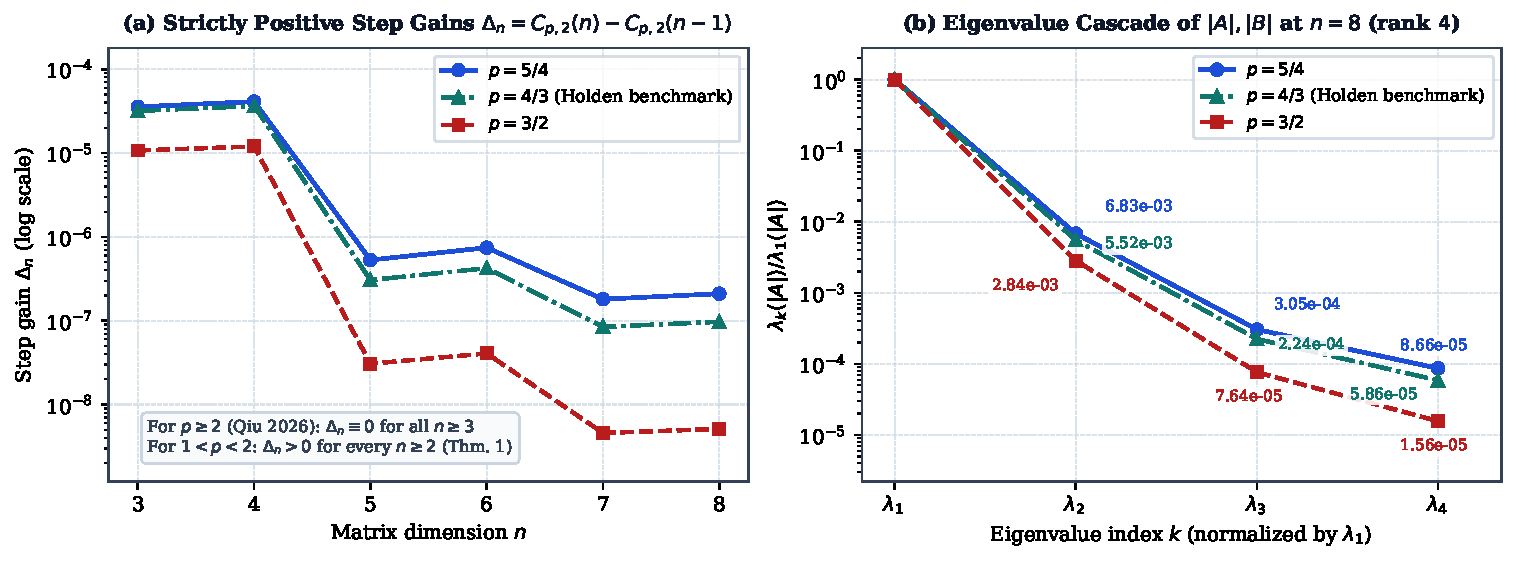
\includegraphics[width=0.98\textwidth]{fig1_staircase_cascade.pdf}
  \vspace{-6pt}
  \caption{\small \emph{Left (a):} Achieved dimensional step gains $\Delta_n = C_{p,2}(n) - C_{p,2}(n-1)$ across $n = 3,\dots,8$ for $p = 5/4$ (blue circles), $p = 4/3$ (teal triangles, Holden's benchmark exponent~\cite{Holden2026b}), and $p = 3/2$ (red squares), contrasting with $p \ge 2$ where $\Delta_n \equiv 0$ for all $n \ge 3$~\cite{Qiu2026}. Notice the paired odd/even plateau structure arising from the alternating rank growth $(1,1)\to(2,1)\to(2,2)\to\cdots$. \emph{Right (b):} Normalized nonzero eigenvalues of $|A|$ (matching $|B|$) at $n = 8$ (rank~$4$), showing rapid geometric decay.}
  \label{fig:cascade}
\end{figure}

\begin{table}[H]
\centering
\caption{\small Achieved lower-bound staircase for $C_{3/2,2}(n)$ across $n = 2,\dots,8$ (Tang--Zhang: $1.0346539519$; Holden interpolated upper bound~\cite{Holden2026b}: $1.04458345$; Theorem~6 $p_0=1, p_1=2$ bound: $1.06475224$).}
\vspace{3pt}
\footnotesize
\begin{tabular}{@{}c c l l l@{}}
\toprule
\textbf{Dim $n$} & \textbf{Ranks ($\rank A, \rank B$)} & \textbf{Achieved ratio} & \textbf{Step gain $\Delta_n$} & \textbf{Normalized nonzero eigenvalues of $|A|$} \\
\midrule
2 & $(1,1)$ & $1.03641435733341^*$ & $+3.641\times 10^{-2}$ & $[1.00]$ \\
3 & $(2,1)$ & $1.03642509117441$   & $+1.073\times 10^{-5}$ & $[1.00,\; 2.47\times 10^{-3}]$ \\
4 & $(2,2)$ & $1.03643708623764$   & $+1.200\times 10^{-5}$ & $[1.00,\; 2.79\times 10^{-3}]$ \\
5 & $(3,2)$ & $1.03643711693849$   & $+3.070\times 10^{-8}$ & $[1.00,\; 2.81\times 10^{-3},\; 5.46\times 10^{-5}]$ \\
6 & $(3,3)$ & $1.03643715767551$   & $+4.074\times 10^{-8}$ & $[1.00,\; 2.84\times 10^{-3},\; 7.63\times 10^{-5}]$ \\
7 & $(4,3)$ & $1.03643716225772$   & $+4.582\times 10^{-9}$ & $[1.00,\; 2.84\times 10^{-3},\; 7.63\times 10^{-5},\; 1.38\times 10^{-5}]$ \\
8 & $(4,4)$ & $1.03643716738222$   & $+5.125\times 10^{-9}$ & $[1.00,\; 2.84\times 10^{-3},\; 7.64\times 10^{-5},\; 1.56\times 10^{-5}]$ \\
\bottomrule
\end{tabular}
\label{tab:p32}
\end{table}

\begin{table}[H]
\centering
\caption{\small Achieved lower-bound staircase for $C_{4/3,2}(n)$ across $n = 2,\dots,8$ (Tang--Zhang: $1.0137583436$; Holden certified enclosure~\cite{Holden2026b}: $1.018371575 < C_{4/3,2}(\infty) \le (861/800)^{1/4} \approx 1.0185404735$).}
\vspace{3pt}
\footnotesize
\begin{tabular}{@{}c c l l l@{}}
\toprule
\textbf{Dim $n$} & \textbf{Ranks ($\rank A, \rank B$)} & \textbf{Achieved ratio} & \textbf{Step gain $\Delta_n$} & \textbf{Normalized nonzero eigenvalues of $|A|$} \\
\midrule
2 & $(1,1)$ & $1.01830237543067^*$ & $+1.830\times 10^{-2}$ & $[1.00]$ \\
3 & $(2,1)$ & $1.01833420141557$   & $+3.183\times 10^{-5}$ & $[1.00,\; 4.38\times 10^{-3}]$ \\
4 & $(2,2)$ & $1.01837064274052$   & $+3.644\times 10^{-5}$ & $[1.00,\; 5.19\times 10^{-3}]$ \\
5 & $(3,2)$ & $1.01837094872573$   & $+3.060\times 10^{-7}$ & $[1.00,\; 5.30\times 10^{-3},\; 1.43\times 10^{-4}]$ \\
6 & $(3,3)$ & $1.01837137193796$   & $+4.232\times 10^{-7}$ & $[1.00,\; 5.48\times 10^{-3},\; 2.22\times 10^{-4}]$ \\
7 & $(4,3)$ & $1.01837145645530$   & $+8.452\times 10^{-8}$ & $[1.00,\; 5.50\times 10^{-3},\; 2.23\times 10^{-4},\; 4.93\times 10^{-5}]$ \\
8 & $(4,4)$ & $1.01837155358673$   & $+9.713\times 10^{-8}$ & $[1.00,\; 5.52\times 10^{-3},\; 2.24\times 10^{-4},\; 5.86\times 10^{-5}]$ \\
\bottomrule
\end{tabular}
\label{tab:p43}
\end{table}

\begin{table}[H]
\centering
\caption{\small Achieved lower-bound staircase for $C_{5/4,2}(n)$ across $n = 2,\dots,8$ (Tang--Zhang: $1.0057587726$; Holden interpolated upper bound~\cite{Holden2026b}: $(861/800)^{1/5} \approx 1.01480508$).}
\vspace{3pt}
\footnotesize
\begin{tabular}{@{}c c l l l@{}}
\toprule
\textbf{Dim $n$} & \textbf{Ranks ($\rank A, \rank B$)} & \textbf{Achieved ratio} & \textbf{Step gain $\Delta_n$} & \textbf{Normalized nonzero eigenvalues of $|A|$} \\
\midrule
2 & $(1,1)$ & $1.01098753445242^*$ & $+1.099\times 10^{-2}$ & $[1.00]$ \\
3 & $(2,1)$ & $1.01102311501737$   & $+3.558\times 10^{-5}$ & $[1.00,\; 5.11\times 10^{-3}]$ \\
4 & $(2,2)$ & $1.01106425559437$   & $+4.114\times 10^{-5}$ & $[1.00,\; 6.21\times 10^{-3}]$ \\
5 & $(3,2)$ & $1.01106478536413$   & $+5.298\times 10^{-7}$ & $[1.00,\; 6.41\times 10^{-3},\; 1.83\times 10^{-4}]$ \\
6 & $(3,3)$ & $1.01106552894231$   & $+7.436\times 10^{-7}$ & $[1.00,\; 6.74\times 10^{-3},\; 3.00\times 10^{-4}]$ \\
7 & $(4,3)$ & $1.01106570953544$   & $+1.806\times 10^{-7}$ & $[1.00,\; 6.78\times 10^{-3},\; 3.03\times 10^{-4},\; 7.09\times 10^{-5}]$ \\
8 & $(4,4)$ & $1.01106591970515$   & $+2.102\times 10^{-7}$ & $[1.00,\; 6.83\times 10^{-3},\; 3.05\times 10^{-4},\; 8.66\times 10^{-5}]$ \\
\bottomrule
\end{tabular}
\label{tab:p54}
\end{table}

\begin{table}[H]
\centering
\caption{\small Extended Theorem~5 PSD-formulation achieved lower-bound staircases ($W_k = Z_k Z_k^\top$, zero unitary variables; \texttt{investigate\_open\_core.py}) through $n = 14$ at $p = 3/2$ and $n = 12$ at $p = 4/3$, confirming pinned top density mass $\lambda_1(T)$ and exact orthogonal-projection defect $\|X_1^2 - X_1\|_F \approx 0$.}
\vspace{3pt}
\footnotesize
\begin{tabular}{@{}c c c l l c c c@{}}
\toprule
\textbf{Exp $p$} & \textbf{Dim $n$} & \textbf{Ranks} & \textbf{Achieved ratio} & \textbf{Even-step gain} & \textbf{Top $\lambda_1(T)$} & \textbf{Min $\lambda_n(T)$} & \textbf{$\|X_1^2 - X_1\|_F$} \\
\midrule
$3/2$ &  8 & $(4,4)$ & $1.036437167382224$ & $+9.707\times 10^{-9}$  & $0.987213$ & $2.20\times 10^{-9}$  & $9.6\times 10^{-12}$ \\
$3/2$ & 10 & $(5,5)$ & $1.036437167985572$ & $+6.033\times 10^{-10}$ & $0.987213$ & $2.12\times 10^{-10}$ & $1.8\times 10^{-11}$ \\
$3/2$ & 12 & $(6,6)$ & $1.036437168024622$ & $+3.905\times 10^{-11}$ & $0.987213$ & $8.86\times 10^{-12}$ & $5.8\times 10^{-10}$ \\
$3/2$ & 14 & $(7,7)$ & $1.036437168055158$ & $+3.054\times 10^{-11}$ & $0.987213$ & $8.62\times 10^{-12}$ & $4.9\times 10^{-9}$  \\
\midrule
$4/3$ &  8 & $(4,4)$ & $1.018371553586731$ & $+1.816\times 10^{-7}$  & $0.966815$ & $2.10\times 10^{-7}$  & $6.0\times 10^{-14}$ \\
$4/3$ & 10 & $(5,5)$ & $1.018371570141039$ & $+1.655\times 10^{-8}$  & $0.966808$ & $3.07\times 10^{-8}$  & $3.1\times 10^{-13}$ \\
$4/3$ & 12 & $(6,6)$ & $1.018371572808177$ & $+2.667\times 10^{-9}$  & $0.966807$ & $3.10\times 10^{-9}$  & $1.1\times 10^{-12}$ \\
\bottomrule
\end{tabular}
\label{tab:psd_ext}
\end{table}

\noindent{\footnotesize\textsuperscript{*}Exact analytical values from Theorem~3. For $m = 3$ at $p = 3/2$, Theorem~3 proves $C_{3/2,3}(2) = C_{3/2,2}(2) \approx 1.036414357333$, while exact-gradient optimization achieves strictly increasing ratios across $n = 2, 3, 4, 5$: $1.036414357333 < 1.063086305441 < 1.063090693728 < 1.063095357075$ (compare Tang--Zhang $C_{3/2,3}^{\TZ} \approx 1.0607584802$). At $p = 4/3$, our $n = 12$ achieved ratio $1.0183715728$ approaches Holden's certified lower bound $1.018371575$~\cite{Holden2026b} from below, consistent with Holden's higher-order cyclic block construction and Theorem~1.}

\subsection{Open-Core Numerical Diagnostics (\texttt{investigate\_open\_core.py})}

Beyond verifying the extended staircases in Table~\ref{tab:psd_ext}, our numerical experiments probe the open structure of MI-20:
\begin{itemize}[leftmargin=1.5em,itemsep=2pt]
  \item \textbf{Continuous-spectrum Hardy/Toeplitz projection test (Open Question~1):} Discretizing multiplication by a density $f(\theta) > 0$ on $\mathbb{T}$ with the Hardy projection $X_1 = P_+$ across $N \in \{32, 64, 128\}$ Fourier modes at $p = 3/2$ gives ratios $\le 1.0054$ (smooth cosine), $\le 1.0154$ (discontinuous step functions), and $\le 1.0297$ (localized spikes), decreasing monotonically with $N$. Direct 6-harmonic optimization at $N = 64$ peaks at $1.032629 < C_{3/2,2}(2) \approx 1.036414$. Together with the remarkably stable top eigenvalue $\lambda_1(T^{(n)}) \approx 0.987213$ ($p = 3/2$) and $0.966807$ ($p = 4/3$) in Table~\ref{tab:psd_ext}, this provides strong exploratory evidence against total spectral vanishing.
  \item \textbf{$p \to 1^+$ quadratic scaling in higher dimensions (resolved by Theorem~10):} Proposition~8 proves the exact limit $\lim_{\varepsilon\to 0^+}(C_{1+\varepsilon,2}(2)-1)/\varepsilon^2 = c_2 \approx 0.21961442$. Optimizing $n = 4$ and $n = 6$ via Theorem~5 at $\varepsilon = 0.01$ achieves $(C_{1.01,2}(4)-1)/\varepsilon^2 = 0.223031$ and $(C_{1.01,2}(6)-1)/\varepsilon^2 = 0.223265$, exceeding $(C_{1.01,2}(2)-1)/\varepsilon^2 = 0.217441$ by $+5.83\times 10^{-3}$, while Theorem~10 now proves the unconditional dimension-free upper bound $\limsup_{\varepsilon\to 0^+}(C_{1+\varepsilon,2}(\infty)-1)/\varepsilon^2 \le K_2 = 0.31723579$.
  \item \textbf{Dual-trace lower bound functional $\Tr(T^\alpha H) / \Tr(T)$ (complementary to Theorem~10):} By H\"older's inequality ($\alpha p' = 1$), $\|H\|_p \ge \Tr(T^\alpha H)$ holds in every dimension $n$ for Theorem~5's canonical form, so any uniform lower bound $\Tr(T^\alpha H) \ge \gamma_{p,m}\Tr(T)$ implies $C_{p,m}(\infty) \le \gamma_{p,m}^{-1}$. Numerically, for $m = 2$, $\min \Tr(T^\alpha H)/\Tr(T)$ stabilizes at $n = 2$ across $n \in \{2, 3, 4, 6\}$ for $p \in \{8/5, 3/2, 7/5\}$—attaining the exact algebraic value $\frac{2\sqrt{2}}{3} \approx 0.94280904$ at $p = 3/2$ (corresponding to $1/\gamma = \frac{3\sqrt{2}}{4} \approx 1.060660$, tighter than Theorem~6's $1.064752$)—while breaking dimensional stabilization below $p \approx 4/3$ ($\alpha = 1/4$) and maintaining quadratic scaling $1 - \gamma_{p,2} \sim \Theta((p-1)^2)$ as $p \to 1^+$ (e.g., $\gamma^{-1} = 1.000559$ at $p = 1.05$, $16\times$ tighter than Theorem~6's $1.00899$).
\end{itemize}

\subsection{Independent Exact-Rational, Symbolic, and 10-Line Verification}

All analytical identities, world-record lower bounds, and Two-State Pinch upper bounds are independently reproduced by our bundled scripts:
\begin{itemize}[leftmargin=1.5em,itemsep=2pt]
  \item \textbf{Zero-float master certificate verifier (\texttt{python3 -B -S verify\_all\_exact\_certificates.py}):} Pure Python 3 standard library (\texttt{fractions}, \texttt{math}, \texttt{json}) with zero floating-point decisions verifies all four suites in under one second: (1)~Theorem~4's three $2\times 3$ witnesses (Weyl radii $\epsilon_H < 1.5\times 10^{-39}$); (2)~Theorem~11's two $42\times 42$ world-record tree lower bounds (\texttt{lower\_record\_certificates.json}, certifying $C_{4/3,2}(\infty) > 1.0183715755$ and $C_{3/2,2}(\infty) > 1.03643716806$); (3)~Theorem~12's 13 four-corner Two-State Pinch upper-bound rectangles (\texttt{upper\_bound\_certificates.json}, checking Theorem~10's exact integer caps, localizer whitelists, seamless parameter coverage, identically zero polynomial residuals, and strictly positive exact rational $LDL^\top$ pivots); and (4)~three negative tamper regression tests plus a literal noncommuting matrix algebra sanity check.
  \item \textbf{Symbolic and 105-digit audit (\texttt{verify\_all\_math.py}):} SymPy checks every derivative factorization, palindromic reduction, and Sturm uniqueness bound in Theorem~3 ($p \in \{3/2, 4/3, 5/4\}$); Lemma~4(a) passes $5{,}000$ random complex PSD matrices ($\max(\mathrm{LHS}-\mathrm{RHS}) = -1.36\times 10^{-9}$); Theorem~3's dual Cauchy--Schwarz bound passes $5{,}000$ random complex tuples; and Lemma~2 strictly increases $\|S\|_p$ on $100/100$ random rank-deficient tuples in 105-digit \texttt{mpmath}.
\end{itemize}

The following self-contained 10-line NumPy snippet reproduces Theorem~4(1) in under one second:
\begin{tcolorbox}[codebox]
\begin{lstlisting}
import numpy as np
p = 1.5
sp = lambda M: np.sum(np.linalg.svd(M, compute_uv=False)**p)**(1/p)
ab = lambda M: (lambda _, s, vt: (vt.T * s) @ vt)(*np.linalg.svd(M, full_matrices=False))
A = np.array([[49., 62., -1.], [11., 14., 0.], [0., 0., 0.]])
B = np.array([[81.,  0.,  0.], [ 0.,  0., 0.], [0., 0., 0.]])
C2 = ((107 + 51*np.sqrt(17)) / 256)**(1/6)  # exact 2x2 supremum (Theorem 3)
ratio = sp(A + B) / sp(ab(A) + ab(B))
print(f"2x2 supremum = {C2:.15f}\n3x3 integer  = {ratio:.15f}\ngap = {ratio - C2:+.3e}")
\end{lstlisting}
\end{tcolorbox}
\vspace{-2pt}
{\ttfamily\footnotesize\color{ink} Output: 2x2 supremum = 1.036414357333407 \;|\; 3x3 integer = 1.036415570430780 \;|\; gap = +1.213e-06.}

\section{Remaining Open Core of Problem MI-20}

With Theorems~1--12, Proposition~5, Proposition~8, the 10-module Lean~4 formalization, and the zero-float master verifier established—including the complete resolution of Version~2's Open Question~2 via Theorem~10's dimension-free quadratic upper bound $\ln C_{p,m}(\infty) \le \frac{m^2-1}{2p^2}(p-1)^2$—the remaining open core of Problem~MI-20 distills to two sharply focused questions:
\begin{enumerate}[leftmargin=1.6em,itemsep=3pt]
  \item \textbf{Exact optimality and analytic evaluation of the infinite-tree fixed point $\Lambda_{\mathrm{tree}}(\infty)$.} At both benchmark exponents $p = 4/3$ and $p = 3/2$ ($m = 2$), our self-similar infinite-tree extremizer (Theorem~11) matches the Two-State Pinch upper bound (Theorem~12) to $6.2 \times 10^{-6}$ and $1.77 \times 10^{-5}$, respectively, and every single-block optimization tested so far obeys the maximal-flux inequality $\phi_{\max}(\Lambda) \le \sigma_+(\Lambda)$ for $\Lambda > \Lambda_{\mathrm{tree}}(\infty)$. Proving that $\Lambda_{\mathrm{tree}}(\infty)$ is the exact global supremum $2^{2\kappa-1} C_{p,m}(\infty)^{2\kappa}$ for all $1 < p < 2$ and $m \ge 2$—and determining whether the transcendental infinite-tree fixed point admits a closed-form analytic expression—remains open.
  \item \textbf{Ruling out total spectral vanishing in Theorem~7.} Proving unconditionally that maximizing sequences in Theorem~5's canonical form satisfy $\limsup_{n\to\infty}\lambda_1(T^{(n)}) > 0$ (as strongly supported by both our stabilized staircases $\lambda_1 \approx 0.9872$ and our trace-class infinite-tree solutions $\sum d_i < 1$) would immediately establish that $C_{p,m}(\infty)$ is attained by a compact infinite-rank tuple in $(\Sp(\ell^2))^m$ obeying the proper co-isometry structure of Theorem~8.
\end{enumerate}

\begin{thebibliography}{11}
\small
\bibitem{Lee2010}
E.-Y. Lee, \emph{Rotfel'd type inequalities for norms}, Linear Algebra and its Applications \textbf{433}(3) (2010), 580--584.

\bibitem{Lee2011}
E.-Y. Lee, \emph{Extension of Rotfel'd theorem}, Linear Algebra and its Applications \textbf{435}(4) (2011), 735--741.

\bibitem{LinZhang2022}
J. Lin and Y. Zhang, \emph{A proof of Lee's conjecture on the sum of absolute values of matrices}, Journal of Mathematical Analysis and Applications \textbf{516} (2022), 126542.

\bibitem{TangZhang2026}
Q. Tang and S. Zhang, \emph{Generalizing Lee's conjecture on the sum of absolute values of matrices}, Linear Algebra and its Applications \textbf{731} (2026), 196--204; arXiv:2510.16846.

\bibitem{Zeng2026}
Z. Zeng, H. Liu, and K. Ratnavelu, \emph{A counterexample to the Tang--Zhang Schatten norm conjecture and sharp positive results}, arXiv:2608.15558 (August 2026).

\bibitem{Qiu2026}
H. Qiu, \emph{Sharp quasi-reverse Minkowski inequality for Schatten norms}, arXiv:2608.17565v2 (August 2026).

\bibitem{Li2026}
X. Li, \emph{Sharp concave-function transfer for Lee-type Schatten norm inequalities}, arXiv:2608.25989v1 (August 2026).

\bibitem{Holden2026a}
S. Holden, \emph{MI-20: dual and projective normal forms}, audited partial-result note archived in \emph{Open Problems in Numerical Linear Algebra} (\nolinkurl{references/holden-matrix-2026-09-12/MI-20/result.md}), September 12, 2026.

\bibitem{Holden2026b}
S. Holden, \emph{MI-20, Round Four: An Exact Universal Bound and a Positive Power-System Reduction}, audited partial-result report archived in \emph{Open Problems in Numerical Linear Algebra} (\nolinkurl{references/holden-continuations-2026-09-13/MI-20/report.pdf}), September 13, 2026.

\bibitem{Davies1988}
E. B. Davies, \emph{Lipschitz continuity of functions of operators in the Schatten classes}, Journal of the London Mathematical Society \textbf{37}(1) (1988), 148--157.

\bibitem{OpenProblemsNLA}
A. Townsend et al., \emph{Open Problems in Numerical Linear Algebra (OpenProblemsInNLA)}, Problem MI-20: \emph{Sharp subquadratic Lee constants for sums of matrices}, \url{https://github.com/ajt60gaibb/OpenProblemsInNLA} (2026).
\end{thebibliography}

\end{document}
